\documentclass[twoside]{book}

% Packages required by doxygen
\usepackage{fixltx2e}
\usepackage{calc}
\usepackage{doxygen}
\usepackage[export]{adjustbox} % also loads graphicx
\usepackage{graphicx}
\usepackage[utf8]{inputenc}
\usepackage{makeidx}
\usepackage{multicol}
\usepackage{multirow}
\PassOptionsToPackage{warn}{textcomp}
\usepackage{textcomp}
\usepackage[nointegrals]{wasysym}
\usepackage[table]{xcolor}

% NLS support packages
\usepackage[french]{babel}

% Font selection
\usepackage[T1]{fontenc}
\usepackage[scaled=.90]{helvet}
\usepackage{courier}
\usepackage{amssymb}
\usepackage{sectsty}
\renewcommand{\familydefault}{\sfdefault}
\allsectionsfont{%
  \fontseries{bc}\selectfont%
  \color{darkgray}%
}
\renewcommand{\DoxyLabelFont}{%
  \fontseries{bc}\selectfont%
  \color{darkgray}%
}
\newcommand{\+}{\discretionary{\mbox{\scriptsize$\hookleftarrow$}}{}{}}

% Page & text layout
\usepackage{geometry}
\geometry{%
  a4paper,%
  top=2.5cm,%
  bottom=2.5cm,%
  left=2.5cm,%
  right=2.5cm%
}
\tolerance=750
\hfuzz=15pt
\hbadness=750
\setlength{\emergencystretch}{15pt}
\setlength{\parindent}{0cm}
\setlength{\parskip}{3ex plus 2ex minus 2ex}
\makeatletter
\renewcommand{\paragraph}{%
  \@startsection{paragraph}{4}{0ex}{-1.0ex}{1.0ex}{%
    \normalfont\normalsize\bfseries\SS@parafont%
  }%
}
\renewcommand{\subparagraph}{%
  \@startsection{subparagraph}{5}{0ex}{-1.0ex}{1.0ex}{%
    \normalfont\normalsize\bfseries\SS@subparafont%
  }%
}
\makeatother

% Headers & footers
\usepackage{fancyhdr}
\pagestyle{fancyplain}
\fancyhead[LE]{\fancyplain{}{\bfseries\thepage}}
\fancyhead[CE]{\fancyplain{}{}}
\fancyhead[RE]{\fancyplain{}{\bfseries\leftmark}}
\fancyhead[LO]{\fancyplain{}{\bfseries\rightmark}}
\fancyhead[CO]{\fancyplain{}{}}
\fancyhead[RO]{\fancyplain{}{\bfseries\thepage}}
\fancyfoot[LE]{\fancyplain{}{}}
\fancyfoot[CE]{\fancyplain{}{}}
\fancyfoot[RE]{\fancyplain{}{\bfseries\scriptsize Généré par Doxygen }}
\fancyfoot[LO]{\fancyplain{}{\bfseries\scriptsize Généré par Doxygen }}
\fancyfoot[CO]{\fancyplain{}{}}
\fancyfoot[RO]{\fancyplain{}{}}
\renewcommand{\footrulewidth}{0.4pt}
\renewcommand{\chaptermark}[1]{%
  \markboth{#1}{}%
}
\renewcommand{\sectionmark}[1]{%
  \markright{\thesection\ #1}%
}

% Indices & bibliography
\usepackage{natbib}
\usepackage[titles]{tocloft}
\setcounter{tocdepth}{3}
\setcounter{secnumdepth}{5}
\makeindex

% Hyperlinks (required, but should be loaded last)
\usepackage{ifpdf}
\ifpdf
  \usepackage[pdftex,pagebackref=true]{hyperref}
\else
  \usepackage[ps2pdf,pagebackref=true]{hyperref}
\fi
\hypersetup{%
  colorlinks=true,%
  linkcolor=blue,%
  citecolor=blue,%
  unicode%
}

% Custom commands
\newcommand{\clearemptydoublepage}{%
  \newpage{\pagestyle{empty}\cleardoublepage}%
}

\usepackage{caption}
\captionsetup{labelsep=space,justification=centering,font={bf},singlelinecheck=off,skip=4pt,position=top}

%===== C O N T E N T S =====

\begin{document}

% Titlepage & ToC
\hypersetup{pageanchor=false,
             bookmarksnumbered=true,
             pdfencoding=unicode
            }
\pagenumbering{roman}
\begin{titlepage}
\vspace*{7cm}
\begin{center}%
{\Large Projet\+Rn }\\
\vspace*{1cm}
{\large Généré par Doxygen 1.8.11}\\
\end{center}
\end{titlepage}
\clearemptydoublepage
\tableofcontents
\clearemptydoublepage
\pagenumbering{arabic}
\hypersetup{pageanchor=true}

%--- Begin generated contents ---
\chapter{Index des classes}
\section{Structures de données}
Liste des structures de données avec une brève description \+:\begin{DoxyCompactList}
\item\contentsline{section}{\hyperlink{structApprentissage}{Apprentissage} \\*Regroupe un couple données d\textquotesingle{}entré et sortie attendue necessaire lors de l\textquotesingle{}apprentissage }{\pageref{structApprentissage}}{}
\item\contentsline{section}{\hyperlink{structBMPHead}{B\+M\+P\+Head} }{\pageref{structBMPHead}}{}
\item\contentsline{section}{\hyperlink{structBMPImHead}{B\+M\+P\+Im\+Head} }{\pageref{structBMPImHead}}{}
\item\contentsline{section}{\hyperlink{structCOUCHE}{C\+O\+U\+C\+HE} \\*Decrit une couche d\textquotesingle{}un réseau de neurone }{\pageref{structCOUCHE}}{}
\item\contentsline{section}{\hyperlink{structImage}{Image} \\*Contient chaque pixel deffinissant une image ainsi que la taille de celle ci }{\pageref{structImage}}{}
\item\contentsline{section}{\hyperlink{structINFO__FENETRE}{I\+N\+F\+O\+\_\+\+F\+E\+N\+E\+T\+RE} \\*Information circulant entre les fonctions }{\pageref{structINFO__FENETRE}}{}
\item\contentsline{section}{\hyperlink{structINFO__RN}{I\+N\+F\+O\+\_\+\+RN} \\*Contient les information concernant un réseau de neurones }{\pageref{structINFO__RN}}{}
\item\contentsline{section}{\hyperlink{structPixel}{Pixel} \\*Definie les composantes rgb d\textquotesingle{}un pixel }{\pageref{structPixel}}{}
\item\contentsline{section}{\hyperlink{structRN}{RN} \\*Defini un réseau de neurones }{\pageref{structRN}}{}
\end{DoxyCompactList}

\chapter{Index des fichiers}
\section{Liste des fichiers}
Liste de tous les fichiers documentés avec une brève description \+:\begin{DoxyCompactList}
\item\contentsline{section}{\hyperlink{Apprentissage_8c}{Apprentissage.\+c} \\*Code de la partie propagation-\/inverse ainsi que toutes les fonctions necessaire a celle ci }{\pageref{Apprentissage_8c}}{}
\item\contentsline{section}{{\bfseries Apprentissage.\+h} }{\pageref{Apprentissage_8h}}{}
\item\contentsline{section}{\hyperlink{gestionnaire__IO_8c}{gestionnaire\+\_\+\+I\+O.\+c} \\*Code des fonctions de lecture et d\textquotesingle{}écriture dans des fichiers }{\pageref{gestionnaire__IO_8c}}{}
\item\contentsline{section}{\hyperlink{gestionnaire__IO_8h}{gestionnaire\+\_\+\+I\+O.\+h} \\*Gestionnaire d\textquotesingle{}entrées sorties }{\pageref{gestionnaire__IO_8h}}{}
\item\contentsline{section}{\hyperlink{gestionnaire__RN_8c}{gestionnaire\+\_\+\+R\+N.\+c} \\*Code de la partie propagation ainsi que toutes les fonctions necessaire a celle ci }{\pageref{gestionnaire__RN_8c}}{}
\item\contentsline{section}{{\bfseries gestionnaire\+\_\+\+R\+N.\+h} }{\pageref{gestionnaire__RN_8h}}{}
\item\contentsline{section}{\hyperlink{interface_8h}{interface.\+h} \\*Interface du programme }{\pageref{interface_8h}}{}
\item\contentsline{section}{{\bfseries neurone.\+h} }{\pageref{neurone_8h}}{}
\item\contentsline{section}{\hyperlink{Structures_8h}{Structures.\+h} \\*Code contenant les structures utilisées dans le programme }{\pageref{Structures_8h}}{}
\item\contentsline{section}{{\bfseries test.\+h} }{\pageref{test_8h}}{}
\end{DoxyCompactList}

\chapter{Documentation des classes}
\hypertarget{structApprentissage}{}\section{Référence de la structure Apprentissage}
\label{structApprentissage}\index{Apprentissage@{Apprentissage}}


Graphe de collaboration de Apprentissage\+:
\nopagebreak
\begin{figure}[H]
\begin{center}
\leavevmode
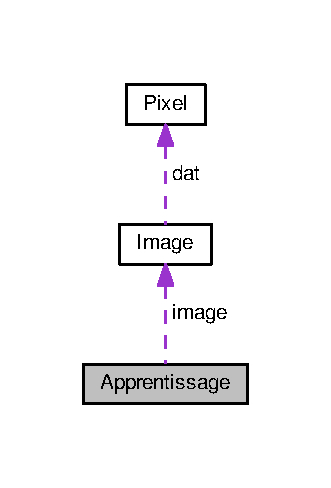
\includegraphics[width=159pt]{structApprentissage__coll__graph}
\end{center}
\end{figure}
\subsection*{Attributs publics}
\begin{DoxyCompactItemize}
\item 
\hyperlink{structImage}{Image} $\ast$ {\bfseries image}\hypertarget{structApprentissage_af3defb9d6e44f5ca0fe145113cec1943}{}\label{structApprentissage_af3defb9d6e44f5ca0fe145113cec1943}

\item 
char $\ast$ {\bfseries etiquette}\hypertarget{structApprentissage_af1668167b1678d621bb9b88573f55be7}{}\label{structApprentissage_af1668167b1678d621bb9b88573f55be7}

\end{DoxyCompactItemize}


La documentation de cette structure a été générée à partir du fichier suivant \+:\begin{DoxyCompactItemize}
\item 
\hyperlink{Structures_8h}{Structures.\+h}\end{DoxyCompactItemize}

\hypertarget{structBMPHead}{}\section{Référence de la structure B\+M\+P\+Head}
\label{structBMPHead}\index{B\+M\+P\+Head@{B\+M\+P\+Head}}


Graphe de collaboration de B\+M\+P\+Head\+:
\nopagebreak
\begin{figure}[H]
\begin{center}
\leavevmode
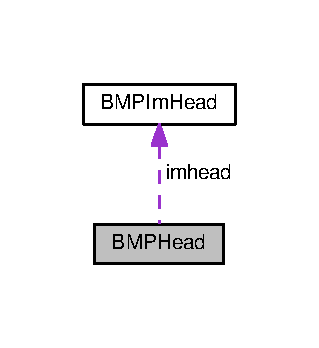
\includegraphics[width=153pt]{structBMPHead__coll__graph}
\end{center}
\end{figure}
\subsection*{Attributs publics}
\begin{DoxyCompactItemize}
\item 
char {\bfseries signature} \mbox{[}2\mbox{]}\hypertarget{structBMPHead_afae656413fe7c6d5c726dcb859003a35}{}\label{structBMPHead_afae656413fe7c6d5c726dcb859003a35}

\item 
int32 {\bfseries taille}\hypertarget{structBMPHead_a129bb82110980f670597d789823f82b4}{}\label{structBMPHead_a129bb82110980f670597d789823f82b4}

\item 
int32 {\bfseries rsv}\hypertarget{structBMPHead_a7b05c13d2a23c9c98854d2ec5249b2d1}{}\label{structBMPHead_a7b05c13d2a23c9c98854d2ec5249b2d1}

\item 
int32 {\bfseries offsetim}\hypertarget{structBMPHead_aadcf34ce8edd039b3314fda48db52a41}{}\label{structBMPHead_aadcf34ce8edd039b3314fda48db52a41}

\item 
struct \hyperlink{structBMPImHead}{B\+M\+P\+Im\+Head} {\bfseries imhead}\hypertarget{structBMPHead_a4a8c172b2b1c554ef3af69e2a80c95d0}{}\label{structBMPHead_a4a8c172b2b1c554ef3af69e2a80c95d0}

\end{DoxyCompactItemize}


La documentation de cette structure a été générée à partir du fichier suivant \+:\begin{DoxyCompactItemize}
\item 
\hyperlink{gestionnaire__IO_8c}{gestionnaire\+\_\+\+I\+O.\+c}\end{DoxyCompactItemize}

\hypertarget{structBMPImHead}{}\section{Référence de la structure B\+M\+P\+Im\+Head}
\label{structBMPImHead}\index{B\+M\+P\+Im\+Head@{B\+M\+P\+Im\+Head}}
\subsection*{Champs de données}
\begin{DoxyCompactItemize}
\item 
int32 {\bfseries size\+\_\+imhead}\hypertarget{structBMPImHead_a087db882c472efd632df406b8bca75aa}{}\label{structBMPImHead_a087db882c472efd632df406b8bca75aa}

\item 
int32 {\bfseries width}\hypertarget{structBMPImHead_ad77d6dd453ad6e0032b53ca9e02bd870}{}\label{structBMPImHead_ad77d6dd453ad6e0032b53ca9e02bd870}

\item 
int32 {\bfseries height}\hypertarget{structBMPImHead_abb7665f76c1c21700df1cd01c4f2fe7d}{}\label{structBMPImHead_abb7665f76c1c21700df1cd01c4f2fe7d}

\item 
int16 {\bfseries nbplans}\hypertarget{structBMPImHead_aa0dc40de38a2d515d99b6fdf7a8b5905}{}\label{structBMPImHead_aa0dc40de38a2d515d99b6fdf7a8b5905}

\item 
int16 {\bfseries bpp}\hypertarget{structBMPImHead_a8ab99ab71fcd3a4bdfbca32b9d68aebc}{}\label{structBMPImHead_a8ab99ab71fcd3a4bdfbca32b9d68aebc}

\item 
int32 {\bfseries compression}\hypertarget{structBMPImHead_a6243975b07502791c6633af57f1026ff}{}\label{structBMPImHead_a6243975b07502791c6633af57f1026ff}

\item 
int32 {\bfseries sizeim}\hypertarget{structBMPImHead_a0ac2156b38e1c53226aafde050189fe0}{}\label{structBMPImHead_a0ac2156b38e1c53226aafde050189fe0}

\item 
int32 {\bfseries hres}\hypertarget{structBMPImHead_a51803597f55adc3bc88a2337e9fb5439}{}\label{structBMPImHead_a51803597f55adc3bc88a2337e9fb5439}

\item 
int32 {\bfseries vres}\hypertarget{structBMPImHead_aa6b95a88db995470ac6ac439db7b1353}{}\label{structBMPImHead_aa6b95a88db995470ac6ac439db7b1353}

\item 
int32 {\bfseries cpalette}\hypertarget{structBMPImHead_a713742cf99ef4cf940950087ba4a4573}{}\label{structBMPImHead_a713742cf99ef4cf940950087ba4a4573}

\item 
int32 {\bfseries c\+Ipalette}\hypertarget{structBMPImHead_a182bbe31daf1af6e415d8c73635caace}{}\label{structBMPImHead_a182bbe31daf1af6e415d8c73635caace}

\end{DoxyCompactItemize}


La documentation de cette structure a été générée à partir du fichier suivant \+:\begin{DoxyCompactItemize}
\item 
gestionnaire\+\_\+\+I\+O.\+c\end{DoxyCompactItemize}

\hypertarget{structCOUCHE}{}\section{Référence de la structure C\+O\+U\+C\+HE}
\label{structCOUCHE}\index{C\+O\+U\+C\+HE@{C\+O\+U\+C\+HE}}


decrit une couche d\textquotesingle{}un réseau de neurone  




{\ttfamily \#include $<$Structures.\+h$>$}



Graphe de collaboration de C\+O\+U\+C\+HE\+:\nopagebreak
\begin{figure}[H]
\begin{center}
\leavevmode
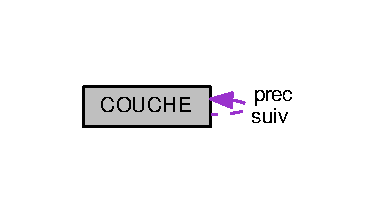
\includegraphics[width=181pt]{structCOUCHE__coll__graph}
\end{center}
\end{figure}
\subsection*{Champs de données}
\begin{DoxyCompactItemize}
\item 
float $\ast$ \hyperlink{structCOUCHE_a2218fee1751e9b8b7355ebe577938f8a}{A}
\item 
float $\ast$ \hyperlink{structCOUCHE_ae39541beb5026e0dc23b79066d841d8a}{B}
\item 
float $\ast$$\ast$ \hyperlink{structCOUCHE_a73df475e85bcea1ab23f681777d2ca2b}{W}
\item 
float $\ast$ \hyperlink{structCOUCHE_a091237265ad9fafe21bad7b8a9cb41e1}{D\+E\+L\+TA}
\item 
float $\ast$$\ast$ \hyperlink{structCOUCHE_ac28815a9c587cba7def4901a7bcfd244}{D\+E\+L\+T\+A\+\_\+M}
\item 
int \hyperlink{structCOUCHE_af841b5acbf63ea3b57522ce796497719}{taille}
\item 
struct \hyperlink{structCOUCHE}{C\+O\+U\+C\+HE} $\ast$ \hyperlink{structCOUCHE_ada93a5c424f0cc1b52d549866ffcd6f9}{prec}
\item 
struct \hyperlink{structCOUCHE}{C\+O\+U\+C\+HE} $\ast$ \hyperlink{structCOUCHE_a17139b5e6dd8e69f1704d902742085cc}{suiv}
\end{DoxyCompactItemize}


\subsection{Description détaillée}
decrit une couche d\textquotesingle{}un réseau de neurone 

\subsection{Documentation des champs}
\index{C\+O\+U\+C\+HE@{C\+O\+U\+C\+HE}!A@{A}}
\index{A@{A}!C\+O\+U\+C\+HE@{C\+O\+U\+C\+HE}}
\subsubsection[{\texorpdfstring{A}{A}}]{\setlength{\rightskip}{0pt plus 5cm}float$\ast$ C\+O\+U\+C\+H\+E\+::A}\hypertarget{structCOUCHE_a2218fee1751e9b8b7355ebe577938f8a}{}\label{structCOUCHE_a2218fee1751e9b8b7355ebe577938f8a}
vecteur des activation de la couche \index{C\+O\+U\+C\+HE@{C\+O\+U\+C\+HE}!B@{B}}
\index{B@{B}!C\+O\+U\+C\+HE@{C\+O\+U\+C\+HE}}
\subsubsection[{\texorpdfstring{B}{B}}]{\setlength{\rightskip}{0pt plus 5cm}float$\ast$ C\+O\+U\+C\+H\+E\+::B}\hypertarget{structCOUCHE_ae39541beb5026e0dc23b79066d841d8a}{}\label{structCOUCHE_ae39541beb5026e0dc23b79066d841d8a}
vecteur des biais de la couche \index{C\+O\+U\+C\+HE@{C\+O\+U\+C\+HE}!D\+E\+L\+TA@{D\+E\+L\+TA}}
\index{D\+E\+L\+TA@{D\+E\+L\+TA}!C\+O\+U\+C\+HE@{C\+O\+U\+C\+HE}}
\subsubsection[{\texorpdfstring{D\+E\+L\+TA}{DELTA}}]{\setlength{\rightskip}{0pt plus 5cm}float$\ast$ C\+O\+U\+C\+H\+E\+::\+D\+E\+L\+TA}\hypertarget{structCOUCHE_a091237265ad9fafe21bad7b8a9cb41e1}{}\label{structCOUCHE_a091237265ad9fafe21bad7b8a9cb41e1}
Vecteur de modification des biais \index{C\+O\+U\+C\+HE@{C\+O\+U\+C\+HE}!D\+E\+L\+T\+A\+\_\+M@{D\+E\+L\+T\+A\+\_\+M}}
\index{D\+E\+L\+T\+A\+\_\+M@{D\+E\+L\+T\+A\+\_\+M}!C\+O\+U\+C\+HE@{C\+O\+U\+C\+HE}}
\subsubsection[{\texorpdfstring{D\+E\+L\+T\+A\+\_\+M}{DELTA_M}}]{\setlength{\rightskip}{0pt plus 5cm}float$\ast$$\ast$ C\+O\+U\+C\+H\+E\+::\+D\+E\+L\+T\+A\+\_\+M}\hypertarget{structCOUCHE_ac28815a9c587cba7def4901a7bcfd244}{}\label{structCOUCHE_ac28815a9c587cba7def4901a7bcfd244}
Matrice de modification des poids \index{C\+O\+U\+C\+HE@{C\+O\+U\+C\+HE}!prec@{prec}}
\index{prec@{prec}!C\+O\+U\+C\+HE@{C\+O\+U\+C\+HE}}
\subsubsection[{\texorpdfstring{prec}{prec}}]{\setlength{\rightskip}{0pt plus 5cm}struct {\bf C\+O\+U\+C\+HE}$\ast$ C\+O\+U\+C\+H\+E\+::prec}\hypertarget{structCOUCHE_ada93a5c424f0cc1b52d549866ffcd6f9}{}\label{structCOUCHE_ada93a5c424f0cc1b52d549866ffcd6f9}
pointeur vers la couche précedente \index{C\+O\+U\+C\+HE@{C\+O\+U\+C\+HE}!suiv@{suiv}}
\index{suiv@{suiv}!C\+O\+U\+C\+HE@{C\+O\+U\+C\+HE}}
\subsubsection[{\texorpdfstring{suiv}{suiv}}]{\setlength{\rightskip}{0pt plus 5cm}struct {\bf C\+O\+U\+C\+HE}$\ast$ C\+O\+U\+C\+H\+E\+::suiv}\hypertarget{structCOUCHE_a17139b5e6dd8e69f1704d902742085cc}{}\label{structCOUCHE_a17139b5e6dd8e69f1704d902742085cc}
pointeur vers la couche suivante \index{C\+O\+U\+C\+HE@{C\+O\+U\+C\+HE}!taille@{taille}}
\index{taille@{taille}!C\+O\+U\+C\+HE@{C\+O\+U\+C\+HE}}
\subsubsection[{\texorpdfstring{taille}{taille}}]{\setlength{\rightskip}{0pt plus 5cm}int C\+O\+U\+C\+H\+E\+::taille}\hypertarget{structCOUCHE_af841b5acbf63ea3b57522ce796497719}{}\label{structCOUCHE_af841b5acbf63ea3b57522ce796497719}
nombre de neurone de la couche \index{C\+O\+U\+C\+HE@{C\+O\+U\+C\+HE}!W@{W}}
\index{W@{W}!C\+O\+U\+C\+HE@{C\+O\+U\+C\+HE}}
\subsubsection[{\texorpdfstring{W}{W}}]{\setlength{\rightskip}{0pt plus 5cm}float$\ast$$\ast$ C\+O\+U\+C\+H\+E\+::W}\hypertarget{structCOUCHE_a73df475e85bcea1ab23f681777d2ca2b}{}\label{structCOUCHE_a73df475e85bcea1ab23f681777d2ca2b}
matrice des poids de la couche 

La documentation de cette structure a été générée à partir du fichier suivant \+:\begin{DoxyCompactItemize}
\item 
\hyperlink{Structures_8h}{Structures.\+h}\end{DoxyCompactItemize}

\hypertarget{structImage}{}\section{Référence de la structure Image}
\label{structImage}\index{Image@{Image}}


Graphe de collaboration de Image\+:
\nopagebreak
\begin{figure}[H]
\begin{center}
\leavevmode
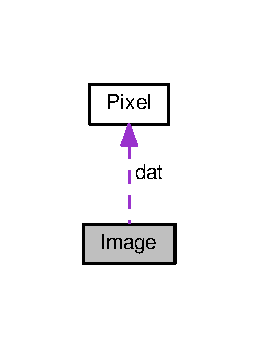
\includegraphics[width=124pt]{structImage__coll__graph}
\end{center}
\end{figure}
\subsection*{Attributs publics}
\begin{DoxyCompactItemize}
\item 
int {\bfseries w}\hypertarget{structImage_a5a1c5528c889b0438bc2dc0c0ee94dbe}{}\label{structImage_a5a1c5528c889b0438bc2dc0c0ee94dbe}

\item 
int {\bfseries h}\hypertarget{structImage_aead13dbc461159381773fff06824e651}{}\label{structImage_aead13dbc461159381773fff06824e651}

\item 
\hyperlink{structPixel}{Pixel} $\ast$ {\bfseries dat}\hypertarget{structImage_abc032a260e391b03f825917716eb07b7}{}\label{structImage_abc032a260e391b03f825917716eb07b7}

\end{DoxyCompactItemize}


La documentation de cette structure a été générée à partir du fichier suivant \+:\begin{DoxyCompactItemize}
\item 
\hyperlink{Structures_8h}{Structures.\+h}\end{DoxyCompactItemize}

\hypertarget{structINFO__FENETRE}{}\section{Référence de la structure I\+N\+F\+O\+\_\+\+F\+E\+N\+E\+T\+RE}
\label{structINFO__FENETRE}\index{I\+N\+F\+O\+\_\+\+F\+E\+N\+E\+T\+RE@{I\+N\+F\+O\+\_\+\+F\+E\+N\+E\+T\+RE}}


Information circulant entre les fonctions.  




{\ttfamily \#include $<$interface.\+h$>$}



Graphe de collaboration de I\+N\+F\+O\+\_\+\+F\+E\+N\+E\+T\+RE\+:
\nopagebreak
\begin{figure}[H]
\begin{center}
\leavevmode
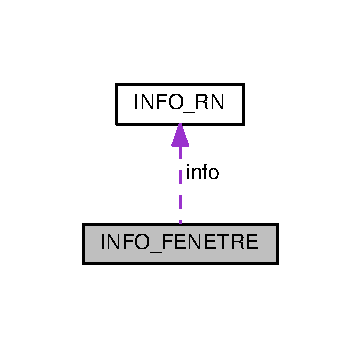
\includegraphics[width=173pt]{structINFO__FENETRE__coll__graph}
\end{center}
\end{figure}
\subsection*{Attributs publics}
\begin{DoxyCompactItemize}
\item 
\hyperlink{structINFO__RN}{I\+N\+F\+O\+\_\+\+RN} $\ast$ \hyperlink{structINFO__FENETRE_a11f9a61d9418b5b167ac2c2dbfa99dac}{info}
\item 
Gtk\+Widget $\ast$ \hyperlink{structINFO__FENETRE_ad55c62f85a92f3163bca921dc73336dc}{Window}
\item 
int \hyperlink{structINFO__FENETRE_ab88f2bbddff749e8003f2b3178fd5602}{nombre\+Reseau}
\item 
int \hyperlink{structINFO__FENETRE_a87ac81a3d0227737e3228bd5ad1f975d}{reseau\+Selectionner}
\item 
char \hyperlink{structINFO__FENETRE_a45ef7a5a1039c09dcb82975b4a070c21}{chemin} \mbox{[}200\mbox{]}
\item 
int \hyperlink{structINFO__FENETRE_ac0a8053617f09b84823e045c847bfdd6}{etat\+Boutton}
\end{DoxyCompactItemize}


\subsection{Description détaillée}
Information circulant entre les fonctions. 

\hyperlink{structINFO__FENETRE}{I\+N\+F\+O\+\_\+\+F\+E\+N\+E\+T\+RE} est un objet de transmission des informations entre les differentes fonction et fenetres. 

\subsection{Documentation des données membres}
\index{I\+N\+F\+O\+\_\+\+F\+E\+N\+E\+T\+RE@{I\+N\+F\+O\+\_\+\+F\+E\+N\+E\+T\+RE}!chemin@{chemin}}
\index{chemin@{chemin}!I\+N\+F\+O\+\_\+\+F\+E\+N\+E\+T\+RE@{I\+N\+F\+O\+\_\+\+F\+E\+N\+E\+T\+RE}}
\subsubsection[{\texorpdfstring{chemin}{chemin}}]{\setlength{\rightskip}{0pt plus 5cm}char I\+N\+F\+O\+\_\+\+F\+E\+N\+E\+T\+R\+E\+::chemin\mbox{[}200\mbox{]}}\hypertarget{structINFO__FENETRE_a45ef7a5a1039c09dcb82975b4a070c21}{}\label{structINFO__FENETRE_a45ef7a5a1039c09dcb82975b4a070c21}
Chemin des fichier ou dossier à enregistrer \index{I\+N\+F\+O\+\_\+\+F\+E\+N\+E\+T\+RE@{I\+N\+F\+O\+\_\+\+F\+E\+N\+E\+T\+RE}!etat\+Boutton@{etat\+Boutton}}
\index{etat\+Boutton@{etat\+Boutton}!I\+N\+F\+O\+\_\+\+F\+E\+N\+E\+T\+RE@{I\+N\+F\+O\+\_\+\+F\+E\+N\+E\+T\+RE}}
\subsubsection[{\texorpdfstring{etat\+Boutton}{etatBoutton}}]{\setlength{\rightskip}{0pt plus 5cm}int I\+N\+F\+O\+\_\+\+F\+E\+N\+E\+T\+R\+E\+::etat\+Boutton}\hypertarget{structINFO__FENETRE_ac0a8053617f09b84823e045c847bfdd6}{}\label{structINFO__FENETRE_ac0a8053617f09b84823e045c847bfdd6}
Etat du boutton \hyperlink{structApprentissage}{Apprentissage} du réseau de neurones \index{I\+N\+F\+O\+\_\+\+F\+E\+N\+E\+T\+RE@{I\+N\+F\+O\+\_\+\+F\+E\+N\+E\+T\+RE}!info@{info}}
\index{info@{info}!I\+N\+F\+O\+\_\+\+F\+E\+N\+E\+T\+RE@{I\+N\+F\+O\+\_\+\+F\+E\+N\+E\+T\+RE}}
\subsubsection[{\texorpdfstring{info}{info}}]{\setlength{\rightskip}{0pt plus 5cm}{\bf I\+N\+F\+O\+\_\+\+RN}$\ast$ I\+N\+F\+O\+\_\+\+F\+E\+N\+E\+T\+R\+E\+::info}\hypertarget{structINFO__FENETRE_a11f9a61d9418b5b167ac2c2dbfa99dac}{}\label{structINFO__FENETRE_a11f9a61d9418b5b167ac2c2dbfa99dac}
Structure contenant tout les Réseaux de neurone existant. \index{I\+N\+F\+O\+\_\+\+F\+E\+N\+E\+T\+RE@{I\+N\+F\+O\+\_\+\+F\+E\+N\+E\+T\+RE}!nombre\+Reseau@{nombre\+Reseau}}
\index{nombre\+Reseau@{nombre\+Reseau}!I\+N\+F\+O\+\_\+\+F\+E\+N\+E\+T\+RE@{I\+N\+F\+O\+\_\+\+F\+E\+N\+E\+T\+RE}}
\subsubsection[{\texorpdfstring{nombre\+Reseau}{nombreReseau}}]{\setlength{\rightskip}{0pt plus 5cm}int I\+N\+F\+O\+\_\+\+F\+E\+N\+E\+T\+R\+E\+::nombre\+Reseau}\hypertarget{structINFO__FENETRE_ab88f2bbddff749e8003f2b3178fd5602}{}\label{structINFO__FENETRE_ab88f2bbddff749e8003f2b3178fd5602}
Nombre de Réseaux de neurones. \index{I\+N\+F\+O\+\_\+\+F\+E\+N\+E\+T\+RE@{I\+N\+F\+O\+\_\+\+F\+E\+N\+E\+T\+RE}!reseau\+Selectionner@{reseau\+Selectionner}}
\index{reseau\+Selectionner@{reseau\+Selectionner}!I\+N\+F\+O\+\_\+\+F\+E\+N\+E\+T\+RE@{I\+N\+F\+O\+\_\+\+F\+E\+N\+E\+T\+RE}}
\subsubsection[{\texorpdfstring{reseau\+Selectionner}{reseauSelectionner}}]{\setlength{\rightskip}{0pt plus 5cm}int I\+N\+F\+O\+\_\+\+F\+E\+N\+E\+T\+R\+E\+::reseau\+Selectionner}\hypertarget{structINFO__FENETRE_a87ac81a3d0227737e3228bd5ad1f975d}{}\label{structINFO__FENETRE_a87ac81a3d0227737e3228bd5ad1f975d}
Réseau sélectionner \index{I\+N\+F\+O\+\_\+\+F\+E\+N\+E\+T\+RE@{I\+N\+F\+O\+\_\+\+F\+E\+N\+E\+T\+RE}!Window@{Window}}
\index{Window@{Window}!I\+N\+F\+O\+\_\+\+F\+E\+N\+E\+T\+RE@{I\+N\+F\+O\+\_\+\+F\+E\+N\+E\+T\+RE}}
\subsubsection[{\texorpdfstring{Window}{Window}}]{\setlength{\rightskip}{0pt plus 5cm}Gtk\+Widget$\ast$ I\+N\+F\+O\+\_\+\+F\+E\+N\+E\+T\+R\+E\+::\+Window}\hypertarget{structINFO__FENETRE_ad55c62f85a92f3163bca921dc73336dc}{}\label{structINFO__FENETRE_ad55c62f85a92f3163bca921dc73336dc}
Fenetre principal qu\textquotesingle{}on modifie dans les fonctions. 

La documentation de cette structure a été générée à partir du fichier suivant \+:\begin{DoxyCompactItemize}
\item 
\hyperlink{interface_8h}{interface.\+h}\end{DoxyCompactItemize}

\hypertarget{structINFO__RN}{}\section{Référence de la structure I\+N\+F\+O\+\_\+\+RN}
\label{structINFO__RN}\index{I\+N\+F\+O\+\_\+\+RN@{I\+N\+F\+O\+\_\+\+RN}}
\subsection*{Attributs publics}
\begin{DoxyCompactItemize}
\item 
char $\ast$$\ast$ {\bfseries etiquettes}\hypertarget{structINFO__RN_abc9704518ac93f743cfebf1baa32a80b}{}\label{structINFO__RN_abc9704518ac93f743cfebf1baa32a80b}

\item 
char $\ast$ {\bfseries nom}\hypertarget{structINFO__RN_a703843a6712fdf0f2b04cd5b809c644c}{}\label{structINFO__RN_a703843a6712fdf0f2b04cd5b809c644c}

\item 
char $\ast$ {\bfseries date}\hypertarget{structINFO__RN_a35f15519beb59c036debb398bb118f46}{}\label{structINFO__RN_a35f15519beb59c036debb398bb118f46}

\item 
char $\ast$ {\bfseries repertoire}\hypertarget{structINFO__RN_a18461fa670221134de73e534b777628c}{}\label{structINFO__RN_a18461fa670221134de73e534b777628c}

\item 
int {\bfseries reussite}\hypertarget{structINFO__RN_a3cab3947c958e59dfe3cee9bc27c2e04}{}\label{structINFO__RN_a3cab3947c958e59dfe3cee9bc27c2e04}

\item 
int {\bfseries echec}\hypertarget{structINFO__RN_a7be6e5b6b85d6f54701cfcb4decf5f4e}{}\label{structINFO__RN_a7be6e5b6b85d6f54701cfcb4decf5f4e}

\item 
int {\bfseries w}\hypertarget{structINFO__RN_a5f950649165382855f5b659f61d75487}{}\label{structINFO__RN_a5f950649165382855f5b659f61d75487}

\item 
int {\bfseries h}\hypertarget{structINFO__RN_ac0d2599d6266859202d791a041f14ae3}{}\label{structINFO__RN_ac0d2599d6266859202d791a041f14ae3}

\end{DoxyCompactItemize}


La documentation de cette structure a été générée à partir du fichier suivant \+:\begin{DoxyCompactItemize}
\item 
\hyperlink{Structures_8h}{Structures.\+h}\end{DoxyCompactItemize}

\hypertarget{structPixel}{}\section{Référence de la structure Pixel}
\label{structPixel}\index{Pixel@{Pixel}}
\subsection*{Attributs publics}
\begin{DoxyCompactItemize}
\item 
unsigned char {\bfseries r}\hypertarget{structPixel_a038ad5b3349e7548d17c5d3bec511b94}{}\label{structPixel_a038ad5b3349e7548d17c5d3bec511b94}

\item 
unsigned char {\bfseries g}\hypertarget{structPixel_a8407845aacf1663d9463475619911686}{}\label{structPixel_a8407845aacf1663d9463475619911686}

\item 
unsigned char {\bfseries b}\hypertarget{structPixel_a760bdf29b15433d257f119239fcff4d4}{}\label{structPixel_a760bdf29b15433d257f119239fcff4d4}

\end{DoxyCompactItemize}


La documentation de cette structure a été générée à partir du fichier suivant \+:\begin{DoxyCompactItemize}
\item 
\hyperlink{Structures_8h}{Structures.\+h}\end{DoxyCompactItemize}

\hypertarget{structRN}{}\section{Référence de la structure RN}
\label{structRN}\index{RN@{RN}}


defini un réseau de neurones  




{\ttfamily \#include $<$Structures.\+h$>$}



Graphe de collaboration de RN\+:\nopagebreak
\begin{figure}[H]
\begin{center}
\leavevmode
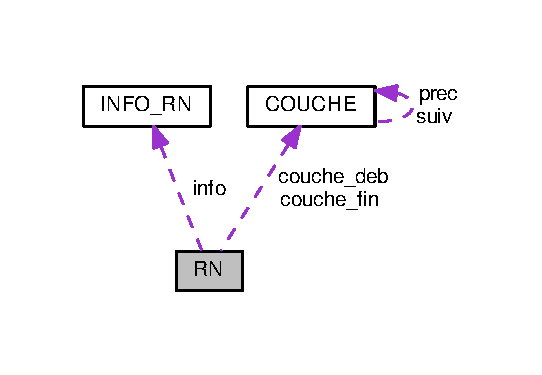
\includegraphics[width=260pt]{structRN__coll__graph}
\end{center}
\end{figure}
\subsection*{Champs de données}
\begin{DoxyCompactItemize}
\item 
\hyperlink{structINFO__RN}{I\+N\+F\+O\+\_\+\+RN} $\ast$ \hyperlink{structRN_a6e638d06aa8ad842d9b7e866f8a0e749}{info}
\item 
\hyperlink{structCOUCHE}{Liste\+\_\+\+Couche} \hyperlink{structRN_a7819ca58c5af68054e17881d5189edb2}{couche\+\_\+deb}
\item 
\hyperlink{structCOUCHE}{Liste\+\_\+\+Couche} \hyperlink{structRN_a587292a48a2d40ee63c00b1e0162e9e2}{couche\+\_\+fin}
\end{DoxyCompactItemize}


\subsection{Description détaillée}
defini un réseau de neurones 

\subsection{Documentation des champs}
\index{RN@{RN}!couche\+\_\+deb@{couche\+\_\+deb}}
\index{couche\+\_\+deb@{couche\+\_\+deb}!RN@{RN}}
\subsubsection[{\texorpdfstring{couche\+\_\+deb}{couche_deb}}]{\setlength{\rightskip}{0pt plus 5cm}{\bf Liste\+\_\+\+Couche} R\+N\+::couche\+\_\+deb}\hypertarget{structRN_a7819ca58c5af68054e17881d5189edb2}{}\label{structRN_a7819ca58c5af68054e17881d5189edb2}
pointeur vers la premiere couche du réseau de neurone \index{RN@{RN}!couche\+\_\+fin@{couche\+\_\+fin}}
\index{couche\+\_\+fin@{couche\+\_\+fin}!RN@{RN}}
\subsubsection[{\texorpdfstring{couche\+\_\+fin}{couche_fin}}]{\setlength{\rightskip}{0pt plus 5cm}{\bf Liste\+\_\+\+Couche} R\+N\+::couche\+\_\+fin}\hypertarget{structRN_a587292a48a2d40ee63c00b1e0162e9e2}{}\label{structRN_a587292a48a2d40ee63c00b1e0162e9e2}
pointeur vers la derniere couche du réseau de neurone \index{RN@{RN}!info@{info}}
\index{info@{info}!RN@{RN}}
\subsubsection[{\texorpdfstring{info}{info}}]{\setlength{\rightskip}{0pt plus 5cm}{\bf I\+N\+F\+O\+\_\+\+RN}$\ast$ R\+N\+::info}\hypertarget{structRN_a6e638d06aa8ad842d9b7e866f8a0e749}{}\label{structRN_a6e638d06aa8ad842d9b7e866f8a0e749}
information du réseau de neurones 

La documentation de cette structure a été générée à partir du fichier suivant \+:\begin{DoxyCompactItemize}
\item 
\hyperlink{Structures_8h}{Structures.\+h}\end{DoxyCompactItemize}

\chapter{Documentation des fichiers}
\hypertarget{Apprentissage_8c}{}\section{Référence du fichier Apprentissage.\+c}
\label{Apprentissage_8c}\index{Apprentissage.\+c@{Apprentissage.\+c}}


Code de la partie propagation-\/inverse ainsi que toutes les fonctions necessaire a celle ci.  


{\ttfamily \#include $<$string.\+h$>$}\\*
{\ttfamily \#include $<$math.\+h$>$}\\*
{\ttfamily \#include $<$stdlib.\+h$>$}\\*
{\ttfamily \#include $<$stdio.\+h$>$}\\*
{\ttfamily \#include \char`\"{}Apprentissage.\+h\char`\"{}}\\*
Graphe des dépendances par inclusion de Apprentissage.\+c\+:
\nopagebreak
\begin{figure}[H]
\begin{center}
\leavevmode
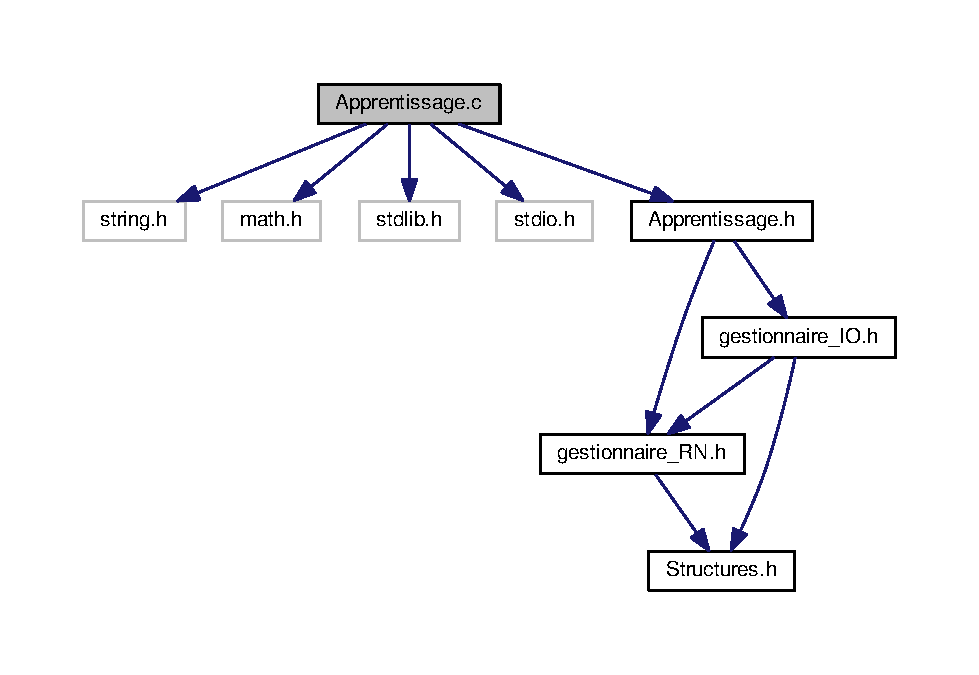
\includegraphics[width=350pt]{Apprentissage_8c__incl}
\end{center}
\end{figure}
\subsection*{Fonctions}
\begin{DoxyCompactItemize}
\item 
void \hyperlink{Apprentissage_8c_ac7e84e7731c88dea339cbed2f65b19d4}{fct\+\_\+cout} (\hyperlink{structRN}{RN} rn, char $\ast$eti)
\begin{DoxyCompactList}\small\item\em sotcke dans le vecteur D\+E\+L\+TA de la derniere couche du réseau la difference entre la valeur obtenue et la valeur souhaitée. \end{DoxyCompactList}\item 
void \hyperlink{Apprentissage_8c_ad11c1cb76d7860d651b3ca20b5c9cb9b}{Back\+Prop} (\hyperlink{structRN}{RN} $\ast$rn, \hyperlink{structImage}{Image} $\ast$im, char $\ast$sortie\+\_\+att, float eta)
\begin{DoxyCompactList}\small\item\em effectue une fois l\textquotesingle{}algorithme de backpropagation sur un réseau de neurone. \end{DoxyCompactList}\item 
void \hyperlink{Apprentissage_8c_a640422ab585eec7089c2d269236f3a85}{Modif\+Poids} (float $\ast$$\ast$W, float $\ast$$\ast$D\+E\+L\+TA, int W\+\_\+w, int W\+\_\+h, float eta)
\begin{DoxyCompactList}\small\item\em modifie les poids d\textquotesingle{}un réseau de neurone \end{DoxyCompactList}\item 
void \hyperlink{Apprentissage_8c_a40e7daf126df4bc4a051b03b22a15e3f}{Modif\+Biais} (float $\ast$B, float $\ast$D\+E\+L\+TA, int taille, float eta)
\begin{DoxyCompactList}\small\item\em modifie les biais d\textquotesingle{}un réseau de neurone \end{DoxyCompactList}\item 
void \hyperlink{Apprentissage_8c_a90d90aaa4be124cafa76914b80ad9321}{Sigmoide\+PrimeZ} (float $\ast$in, float $\ast$$\ast$out, int taille)
\begin{DoxyCompactList}\small\item\em effectue le calcul a$\ast$(1-\/a) \end{DoxyCompactList}\item 
void \hyperlink{Apprentissage_8c_acb686b6abf78231e095fc83947b2ba82}{Multiplication\+Matricielle\+Transposee\+TM} (float $\ast$$\ast$in\+\_\+M, float $\ast$in\+\_\+V, float $\ast$out, int taille\+\_\+\+M1, int taille\+\_\+\+M3)
\begin{DoxyCompactList}\small\item\em effectue une multiplication matricielle en transposant la premiere matrice \end{DoxyCompactList}\item 
void {\bfseries Multiplication\+Matricielle\+Transposee\+MT} (float $\ast$in\+\_\+\+M1, float $\ast$in\+\_\+\+M2, float $\ast$$\ast$out, int taille\+\_\+\+M1, int taille\+\_\+\+M2)\hypertarget{Apprentissage_8c_acc6059e44e95f6e4f51ced681c175255}{}\label{Apprentissage_8c_acc6059e44e95f6e4f51ced681c175255}

\item 
void \hyperlink{Apprentissage_8c_ad3feb851d99301e70423a23fdee859a2}{Hadamard} (float $\ast$$\ast$in\+\_\+a, float $\ast$in\+\_\+b, float $\ast$out, int taille)
\begin{DoxyCompactList}\small\item\em effectue le produit hadamard \end{DoxyCompactList}\item 
void \hyperlink{Apprentissage_8c_a1dda906c280f7d02dcf562cd554e17e8}{Del\+App} (\hyperlink{structApprentissage}{App} $\ast$app)
\begin{DoxyCompactList}\small\item\em libere la mémoire d\textquotesingle{}une structure App \end{DoxyCompactList}\end{DoxyCompactItemize}


\subsection{Description détaillée}
Code de la partie propagation-\/inverse ainsi que toutes les fonctions necessaire a celle ci. 

\begin{DoxyAuthor}{Auteur}
P\+E\+P\+IN Thibaut 

R\+E\+Z\+G\+UI Soumia 

S\+L\+I\+M\+A\+NI Arezki 

S\+E\+L\+A\+Q\+U\+ET Severine 

S\+Z\+U\+L\+EK Isaac 

M\+O\+N\+T\+I\+G\+N\+ET Anthony 
\end{DoxyAuthor}


\subsection{Documentation des fonctions}
\index{Apprentissage.\+c@{Apprentissage.\+c}!Back\+Prop@{Back\+Prop}}
\index{Back\+Prop@{Back\+Prop}!Apprentissage.\+c@{Apprentissage.\+c}}
\subsubsection[{\texorpdfstring{Back\+Prop(\+R\+N $\ast$rn, Image $\ast$im, char $\ast$sortie\+\_\+att, float eta)}{BackProp(RN *rn, Image *im, char *sortie_att, float eta)}}]{\setlength{\rightskip}{0pt plus 5cm}void Back\+Prop (
\begin{DoxyParamCaption}
\item[{{\bf RN} $\ast$}]{rn, }
\item[{{\bf Image} $\ast$}]{im, }
\item[{char $\ast$}]{sortie\+\_\+att, }
\item[{float}]{eta}
\end{DoxyParamCaption}
)}\hypertarget{Apprentissage_8c_ad11c1cb76d7860d651b3ca20b5c9cb9b}{}\label{Apprentissage_8c_ad11c1cb76d7860d651b3ca20b5c9cb9b}


effectue une fois l\textquotesingle{}algorithme de backpropagation sur un réseau de neurone. 


\begin{DoxyParams}{Paramètres}
{\em rn} & le réseau de neurones \\
\hline
{\em im} & l\textquotesingle{}image a fournir comme donnée d\textquotesingle{}entré au réseau de neurones \\
\hline
{\em sortie\+\_\+att} & l\textquotesingle{}etiquette attendu correspondant a l\textquotesingle{}image fournie \\
\hline
{\em eta} & le taux d\textquotesingle{}apprentissage \\
\hline
\end{DoxyParams}
\index{Apprentissage.\+c@{Apprentissage.\+c}!Del\+App@{Del\+App}}
\index{Del\+App@{Del\+App}!Apprentissage.\+c@{Apprentissage.\+c}}
\subsubsection[{\texorpdfstring{Del\+App(\+App $\ast$app)}{DelApp(App *app)}}]{\setlength{\rightskip}{0pt plus 5cm}void Del\+App (
\begin{DoxyParamCaption}
\item[{{\bf App} $\ast$}]{app}
\end{DoxyParamCaption}
)}\hypertarget{Apprentissage_8c_a1dda906c280f7d02dcf562cd554e17e8}{}\label{Apprentissage_8c_a1dda906c280f7d02dcf562cd554e17e8}


libere la mémoire d\textquotesingle{}une structure App 


\begin{DoxyParams}{Paramètres}
{\em app} & élément a liberer de la mémoire \\
\hline
\end{DoxyParams}
\index{Apprentissage.\+c@{Apprentissage.\+c}!fct\+\_\+cout@{fct\+\_\+cout}}
\index{fct\+\_\+cout@{fct\+\_\+cout}!Apprentissage.\+c@{Apprentissage.\+c}}
\subsubsection[{\texorpdfstring{fct\+\_\+cout(\+R\+N rn, char $\ast$eti)}{fct_cout(RN rn, char *eti)}}]{\setlength{\rightskip}{0pt plus 5cm}void fct\+\_\+cout (
\begin{DoxyParamCaption}
\item[{{\bf RN}}]{rn, }
\item[{char $\ast$}]{eti}
\end{DoxyParamCaption}
)}\hypertarget{Apprentissage_8c_ac7e84e7731c88dea339cbed2f65b19d4}{}\label{Apprentissage_8c_ac7e84e7731c88dea339cbed2f65b19d4}


sotcke dans le vecteur D\+E\+L\+TA de la derniere couche du réseau la difference entre la valeur obtenue et la valeur souhaitée. 


\begin{DoxyParams}{Paramètres}
{\em rn} & le réseau de neurones \\
\hline
{\em eti} & l\textquotesingle{}etiquette attendue \\
\hline
\end{DoxyParams}
\index{Apprentissage.\+c@{Apprentissage.\+c}!Hadamard@{Hadamard}}
\index{Hadamard@{Hadamard}!Apprentissage.\+c@{Apprentissage.\+c}}
\subsubsection[{\texorpdfstring{Hadamard(float $\ast$$\ast$in\+\_\+a, float $\ast$in\+\_\+b, float $\ast$out, int taille)}{Hadamard(float **in_a, float *in_b, float *out, int taille)}}]{\setlength{\rightskip}{0pt plus 5cm}void Hadamard (
\begin{DoxyParamCaption}
\item[{float $\ast$$\ast$}]{in\+\_\+a, }
\item[{float $\ast$}]{in\+\_\+b, }
\item[{float $\ast$}]{out, }
\item[{int}]{taille}
\end{DoxyParamCaption}
)}\hypertarget{Apprentissage_8c_ad3feb851d99301e70423a23fdee859a2}{}\label{Apprentissage_8c_ad3feb851d99301e70423a23fdee859a2}


effectue le produit hadamard 


\begin{DoxyParams}{Paramètres}
{\em in\+\_\+a} & premier vecteur de l\textquotesingle{}opération \\
\hline
{\em in\+\_\+b} & deuxieme vecteur de l\textquotesingle{}opération \\
\hline
{\em out} & vecteur ou sera stocké le résultat \\
\hline
{\em taille} & taille du vecteur d\textquotesingle{}entrée \\
\hline
\end{DoxyParams}
\index{Apprentissage.\+c@{Apprentissage.\+c}!Modif\+Biais@{Modif\+Biais}}
\index{Modif\+Biais@{Modif\+Biais}!Apprentissage.\+c@{Apprentissage.\+c}}
\subsubsection[{\texorpdfstring{Modif\+Biais(float $\ast$\+B, float $\ast$\+D\+E\+L\+T\+A, int taille, float eta)}{ModifBiais(float *B, float *DELTA, int taille, float eta)}}]{\setlength{\rightskip}{0pt plus 5cm}void Modif\+Biais (
\begin{DoxyParamCaption}
\item[{float $\ast$}]{B, }
\item[{float $\ast$}]{D\+E\+L\+TA, }
\item[{int}]{taille, }
\item[{float}]{eta}
\end{DoxyParamCaption}
)}\hypertarget{Apprentissage_8c_a40e7daf126df4bc4a051b03b22a15e3f}{}\label{Apprentissage_8c_a40e7daf126df4bc4a051b03b22a15e3f}


modifie les biais d\textquotesingle{}un réseau de neurone 


\begin{DoxyParams}{Paramètres}
{\em B} & le vecteur des biais d\textquotesingle{}un réseau de neurone \\
\hline
{\em D\+E\+L\+TA} & les modifications a apporter \\
\hline
{\em taille} & taille du vecteur B \\
\hline
{\em eta} & taux d\textquotesingle{}apprentissage \\
\hline
\end{DoxyParams}
\index{Apprentissage.\+c@{Apprentissage.\+c}!Modif\+Poids@{Modif\+Poids}}
\index{Modif\+Poids@{Modif\+Poids}!Apprentissage.\+c@{Apprentissage.\+c}}
\subsubsection[{\texorpdfstring{Modif\+Poids(float $\ast$$\ast$\+W, float $\ast$$\ast$\+D\+E\+L\+T\+A, int W\+\_\+w, int W\+\_\+h, float eta)}{ModifPoids(float **W, float **DELTA, int W_w, int W_h, float eta)}}]{\setlength{\rightskip}{0pt plus 5cm}void Modif\+Poids (
\begin{DoxyParamCaption}
\item[{float $\ast$$\ast$}]{W, }
\item[{float $\ast$$\ast$}]{D\+E\+L\+TA, }
\item[{int}]{W\+\_\+w, }
\item[{int}]{W\+\_\+h, }
\item[{float}]{eta}
\end{DoxyParamCaption}
)}\hypertarget{Apprentissage_8c_a640422ab585eec7089c2d269236f3a85}{}\label{Apprentissage_8c_a640422ab585eec7089c2d269236f3a85}


modifie les poids d\textquotesingle{}un réseau de neurone 


\begin{DoxyParams}{Paramètres}
{\em W} & la matrice des poids d\textquotesingle{}un réseau de neurone \\
\hline
{\em D\+E\+L\+TA} & les modifications a apporter \\
\hline
{\em W\+\_\+w} & largeur de W \\
\hline
{\em W\+\_\+h} & hauteur de W \\
\hline
{\em eta} & taux d\textquotesingle{}apprentissage \\
\hline
\end{DoxyParams}
\index{Apprentissage.\+c@{Apprentissage.\+c}!Multiplication\+Matricielle\+Transposee\+TM@{Multiplication\+Matricielle\+Transposee\+TM}}
\index{Multiplication\+Matricielle\+Transposee\+TM@{Multiplication\+Matricielle\+Transposee\+TM}!Apprentissage.\+c@{Apprentissage.\+c}}
\subsubsection[{\texorpdfstring{Multiplication\+Matricielle\+Transposee\+T\+M(float $\ast$$\ast$in\+\_\+\+M, float $\ast$in\+\_\+\+V, float $\ast$out, int taille\+\_\+\+M1, int taille\+\_\+\+M3)}{MultiplicationMatricielleTransposeeTM(float **in_M, float *in_V, float *out, int taille_M1, int taille_M3)}}]{\setlength{\rightskip}{0pt plus 5cm}void Multiplication\+Matricielle\+Transposee\+TM (
\begin{DoxyParamCaption}
\item[{float $\ast$$\ast$}]{in\+\_\+M, }
\item[{float $\ast$}]{in\+\_\+V, }
\item[{float $\ast$}]{out, }
\item[{int}]{taille\+\_\+\+M1, }
\item[{int}]{taille\+\_\+\+M3}
\end{DoxyParamCaption}
)}\hypertarget{Apprentissage_8c_acb686b6abf78231e095fc83947b2ba82}{}\label{Apprentissage_8c_acb686b6abf78231e095fc83947b2ba82}


effectue une multiplication matricielle en transposant la premiere matrice 

effectue une multiplication matricielle en transposant la deuxieme matrice (qui est un vecteur)


\begin{DoxyParams}{Paramètres}
{\em in\+\_\+M} & premiere matrice du calcul, sera transposée avant d\textquotesingle{}etre multipliée \\
\hline
{\em in\+\_\+V} & vecteur qui sera multiplié a la matrice \\
\hline
{\em out} & vecteur ou sera stocké le résultat \\
\hline
{\em taille\+\_\+\+M1} & largeur de la matrice \\
\hline
{\em taille\+\_\+\+M3} & hauteur de la matrice\\
\hline
{\em in\+\_\+M} & premiere matrice du calcul \\
\hline
{\em in\+\_\+V} & vecteur, sera transposée avant d\textquotesingle{}etre multipliée a la matrice \\
\hline
{\em out} & vecteur ou sera stocké le résultat \\
\hline
{\em taille\+\_\+\+M1} & hauteur de la matrice \\
\hline
{\em taille\+\_\+\+M3} & largeur de la matrice \\
\hline
\end{DoxyParams}
\index{Apprentissage.\+c@{Apprentissage.\+c}!Sigmoide\+PrimeZ@{Sigmoide\+PrimeZ}}
\index{Sigmoide\+PrimeZ@{Sigmoide\+PrimeZ}!Apprentissage.\+c@{Apprentissage.\+c}}
\subsubsection[{\texorpdfstring{Sigmoide\+Prime\+Z(float $\ast$in, float $\ast$$\ast$out, int taille)}{SigmoidePrimeZ(float *in, float **out, int taille)}}]{\setlength{\rightskip}{0pt plus 5cm}void Sigmoide\+PrimeZ (
\begin{DoxyParamCaption}
\item[{float $\ast$}]{in, }
\item[{float $\ast$$\ast$}]{out, }
\item[{int}]{taille}
\end{DoxyParamCaption}
)}\hypertarget{Apprentissage_8c_a90d90aaa4be124cafa76914b80ad9321}{}\label{Apprentissage_8c_a90d90aaa4be124cafa76914b80ad9321}


effectue le calcul a$\ast$(1-\/a) 


\begin{DoxyParams}{Paramètres}
{\em in} & vecteur d\textquotesingle{}entrée \\
\hline
{\em out} & vecteur de sortie \\
\hline
{\em taille} & taille du vecteur d\textquotesingle{}entrée \\
\hline
\end{DoxyParams}

\hypertarget{gestionnaire__IO_8c}{}\section{Référence du fichier gestionnaire\+\_\+\+I\+O.\+c}
\label{gestionnaire__IO_8c}\index{gestionnaire\+\_\+\+I\+O.\+c@{gestionnaire\+\_\+\+I\+O.\+c}}


Code des fonctions de lecture et d\textquotesingle{}écriture dans des fichiers.  


{\ttfamily \#include $<$stdio.\+h$>$}\\*
{\ttfamily \#include $<$stdlib.\+h$>$}\\*
{\ttfamily \#include $<$string.\+h$>$}\\*
{\ttfamily \#include $<$assert.\+h$>$}\\*
{\ttfamily \#include $<$sys/types.\+h$>$}\\*
{\ttfamily \#include $<$dirent.\+h$>$}\\*
{\ttfamily \#include $<$sys/dir.\+h$>$}\\*
{\ttfamily \#include $<$errno.\+h$>$}\\*
{\ttfamily \#include $<$sys/stat.\+h$>$}\\*
{\ttfamily \#include $<$stdint.\+h$>$}\\*
{\ttfamily \#include $<$inttypes.\+h$>$}\\*
{\ttfamily \#include $<$unistd.\+h$>$}\\*
{\ttfamily \#include \char`\"{}gestionnaire\+\_\+\+I\+O.\+h\char`\"{}}\\*
Graphe des dépendances par inclusion de gestionnaire\+\_\+\+I\+O.\+c\+:
\nopagebreak
\begin{figure}[H]
\begin{center}
\leavevmode
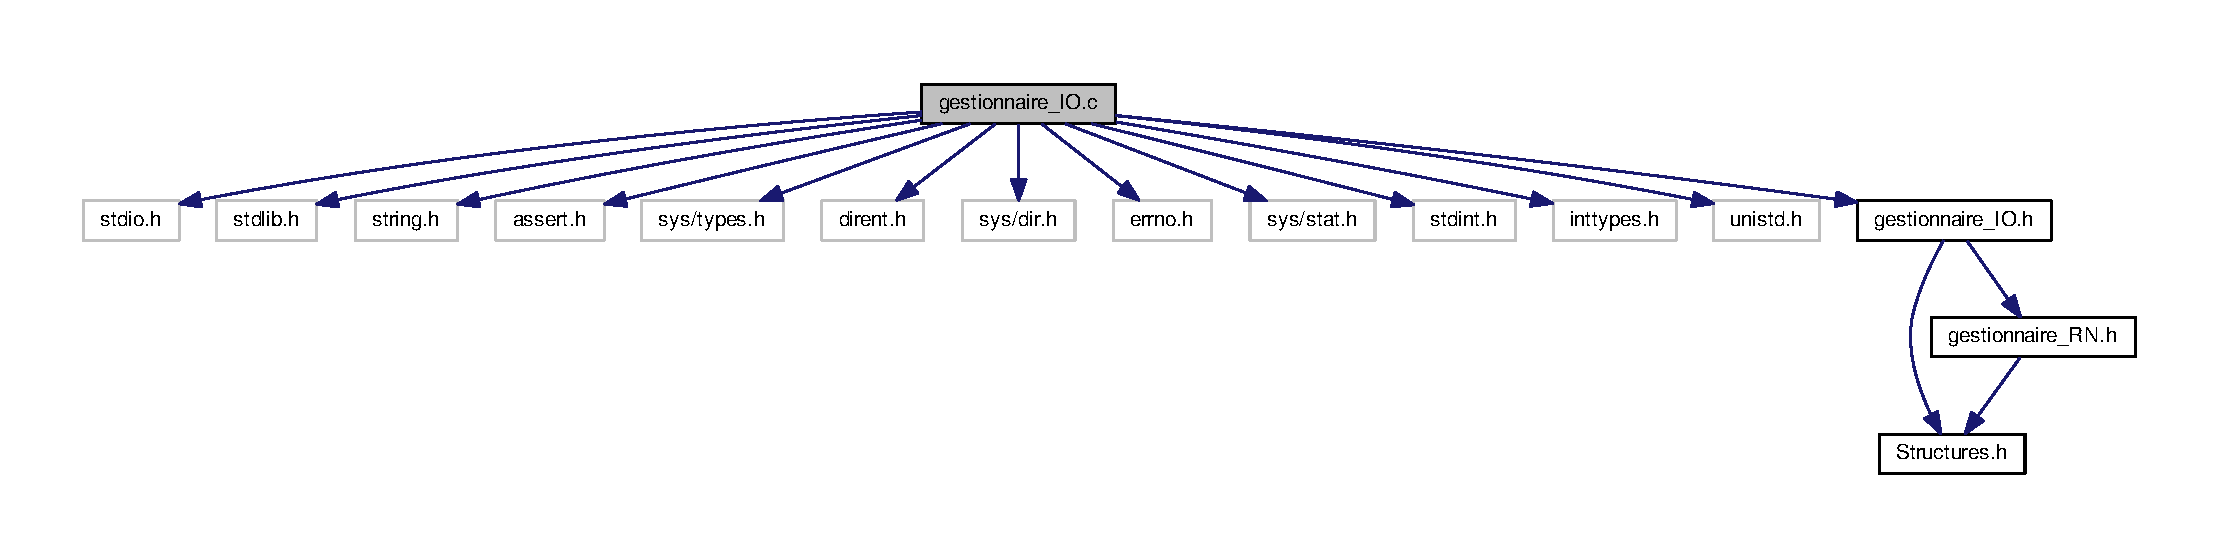
\includegraphics[width=350pt]{gestionnaire__IO_8c__incl}
\end{center}
\end{figure}
\subsection*{Classes}
\begin{DoxyCompactItemize}
\item 
struct \hyperlink{structBMPImHead}{B\+M\+P\+Im\+Head}
\item 
struct \hyperlink{structBMPHead}{B\+M\+P\+Head}
\end{DoxyCompactItemize}
\subsection*{Macros}
\begin{DoxyCompactItemize}
\item 
\#define {\bfseries \+\_\+\+C\+R\+T\+\_\+\+S\+E\+C\+U\+R\+E\+\_\+\+N\+O\+\_\+\+W\+A\+R\+N\+I\+N\+GS}\hypertarget{gestionnaire__IO_8c_af08ec37a8c99d747fb60fa15bc28678b}{}\label{gestionnaire__IO_8c_af08ec37a8c99d747fb60fa15bc28678b}

\item 
\#define {\bfseries debug}~printf(\char`\"{}line \+: \%d in function \+: \%s in file \%s\textbackslash{}n\char`\"{},\+\_\+\+\_\+\+L\+I\+N\+E\+\_\+\+\_\+,\+\_\+\+\_\+func\+\_\+\+\_\+,\+\_\+\+\_\+\+F\+I\+L\+E\+\_\+\+\_\+);\hypertarget{gestionnaire__IO_8c_a322565ccf348d13e4d3de13af771e5fc}{}\label{gestionnaire__IO_8c_a322565ccf348d13e4d3de13af771e5fc}

\end{DoxyCompactItemize}
\subsection*{Définitions de type}
\begin{DoxyCompactItemize}
\item 
typedef int {\bfseries int32}\hypertarget{gestionnaire__IO_8c_a56f1a81c92849566ae864511088eb7e8}{}\label{gestionnaire__IO_8c_a56f1a81c92849566ae864511088eb7e8}

\item 
typedef short {\bfseries int16}\hypertarget{gestionnaire__IO_8c_a4355d16fcf9f644c9ac84293f0b1801f}{}\label{gestionnaire__IO_8c_a4355d16fcf9f644c9ac84293f0b1801f}

\end{DoxyCompactItemize}
\subsection*{Fonctions}
\begin{DoxyCompactItemize}
\item 
\hyperlink{structImage}{Image} $\ast$ {\bfseries Nouvelle\+Image} (int w, int h)\hypertarget{gestionnaire__IO_8c_ac91839d8b84692804f4b60afe1bb216f}{}\label{gestionnaire__IO_8c_ac91839d8b84692804f4b60afe1bb216f}

\item 
\hyperlink{structImage}{Image} $\ast$ {\bfseries Copie\+Image} (\hyperlink{structImage}{Image} $\ast$I)\hypertarget{gestionnaire__IO_8c_ad36403c11915b551d750b94d617af620}{}\label{gestionnaire__IO_8c_ad36403c11915b551d750b94d617af620}

\item 
void {\bfseries Del\+Image} (\hyperlink{structImage}{Image} $\ast$I)\hypertarget{gestionnaire__IO_8c_a05735abfbf6d85ac173e89bea1bf8292}{}\label{gestionnaire__IO_8c_a05735abfbf6d85ac173e89bea1bf8292}

\item 
void {\bfseries Set\+Pixel} (\hyperlink{structImage}{Image} $\ast$I, int i, int j, \hyperlink{structPixel}{Pixel} p)\hypertarget{gestionnaire__IO_8c_a5e175e9510f61a53471ec283ee2c8e56}{}\label{gestionnaire__IO_8c_a5e175e9510f61a53471ec283ee2c8e56}

\item 
\hyperlink{structPixel}{Pixel} {\bfseries Get\+Pixel} (\hyperlink{structImage}{Image} $\ast$I, int i, int j)\hypertarget{gestionnaire__IO_8c_a45c2e01712f3b36fdc1becde80c8356f}{}\label{gestionnaire__IO_8c_a45c2e01712f3b36fdc1becde80c8356f}

\item 
\hyperlink{structImage}{Image} $\ast$ \hyperlink{gestionnaire__IO_8c_a736f28efdaaa51977fd9045eb5b92f91}{Charger\+Bmp} (const char $\ast$fichier, int w\+\_\+max, int h\+\_\+max)
\begin{DoxyCompactList}\small\item\em On lis une image de format bmp et on l\textquotesingle{}enregistre dans la structure \hyperlink{structImage}{Image}. \end{DoxyCompactList}\item 
int {\bfseries Sauver} (\hyperlink{structImage}{Image} $\ast$I, const char $\ast$fichier)\hypertarget{gestionnaire__IO_8c_afea85431922f70840e9d0801f2f57542}{}\label{gestionnaire__IO_8c_afea85431922f70840e9d0801f2f57542}

\item 
\hyperlink{structImage}{Image} $\ast$ {\bfseries Charger\+Mnist} (const char $\ast$path, int w\+\_\+max, int h\+\_\+max)\hypertarget{gestionnaire__IO_8c_a87f6d34e630e1b4d6053be54b2511f03}{}\label{gestionnaire__IO_8c_a87f6d34e630e1b4d6053be54b2511f03}

\item 
char $\ast$ {\bfseries Charger\+Etiquette\+M\+N\+I\+ST} (const char $\ast$path)\hypertarget{gestionnaire__IO_8c_ad75487d79bfcd9c86941964341b27ed4}{}\label{gestionnaire__IO_8c_ad75487d79bfcd9c86941964341b27ed4}

\item 
\hyperlink{structApprentissage}{App} $\ast$ {\bfseries Chargement\+Couple\+Att\+In} (char $\ast$repertoire\+\_\+app, int w\+\_\+max, int h\+\_\+max)\hypertarget{gestionnaire__IO_8c_af173f0494a794123f2c65871af91ef8b}{}\label{gestionnaire__IO_8c_af173f0494a794123f2c65871af91ef8b}

\item 
\hyperlink{structINFO__RN}{I\+N\+F\+O\+\_\+\+RN} $\ast$ {\bfseries Charger\+Info} ()\hypertarget{gestionnaire__IO_8c_a343472a40d9ee1ed25bb7caf22be1b8f}{}\label{gestionnaire__IO_8c_a343472a40d9ee1ed25bb7caf22be1b8f}

\item 
\hyperlink{structRN}{RN} $\ast$ {\bfseries Charger\+RN} (\hyperlink{structINFO__RN}{I\+N\+F\+O\+\_\+\+RN} $\ast$info)\hypertarget{gestionnaire__IO_8c_af2e5b9ad00cab116ec82a35aa1e1c7f0}{}\label{gestionnaire__IO_8c_af2e5b9ad00cab116ec82a35aa1e1c7f0}

\item 
void {\bfseries Save\+RN} (\hyperlink{structRN}{RN} rn)\hypertarget{gestionnaire__IO_8c_a31712d225439b4d860c5770ceb6ddbc9}{}\label{gestionnaire__IO_8c_a31712d225439b4d860c5770ceb6ddbc9}

\end{DoxyCompactItemize}


\subsection{Description détaillée}
Code des fonctions de lecture et d\textquotesingle{}écriture dans des fichiers. 

\begin{DoxyAuthor}{Auteur}
P\+E\+P\+IN Thibaut 

R\+E\+Z\+G\+UI Soumia 

S\+L\+I\+M\+A\+NI Arezki 

S\+E\+L\+A\+Q\+U\+ET Severine 

S\+Z\+U\+L\+EK Isaac 

M\+O\+N\+T\+I\+G\+N\+ET Anthony 
\end{DoxyAuthor}


\subsection{Documentation des fonctions}
\index{gestionnaire\+\_\+\+I\+O.\+c@{gestionnaire\+\_\+\+I\+O.\+c}!Charger\+Bmp@{Charger\+Bmp}}
\index{Charger\+Bmp@{Charger\+Bmp}!gestionnaire\+\_\+\+I\+O.\+c@{gestionnaire\+\_\+\+I\+O.\+c}}
\subsubsection[{\texorpdfstring{Charger\+Bmp(const char $\ast$fichier, int w\+\_\+max, int h\+\_\+max)}{ChargerBmp(const char *fichier, int w_max, int h_max)}}]{\setlength{\rightskip}{0pt plus 5cm}{\bf Image} $\ast$ Charger\+Bmp (
\begin{DoxyParamCaption}
\item[{const char $\ast$}]{fichier, }
\item[{int}]{w\+\_\+max, }
\item[{int}]{h\+\_\+max}
\end{DoxyParamCaption}
)}\hypertarget{gestionnaire__IO_8c_a736f28efdaaa51977fd9045eb5b92f91}{}\label{gestionnaire__IO_8c_a736f28efdaaa51977fd9045eb5b92f91}


On lis une image de format bmp et on l\textquotesingle{}enregistre dans la structure \hyperlink{structImage}{Image}. 


\begin{DoxyParams}{Paramètres}
{\em fichier} & Chemin absolue de l\textquotesingle{}image à charger. \\
\hline
{\em } & \\
\hline
\end{DoxyParams}

\hypertarget{gestionnaire__IO_8h}{}\section{Référence du fichier gestionnaire\+\_\+\+I\+O.\+h}
\label{gestionnaire__IO_8h}\index{gestionnaire\+\_\+\+I\+O.\+h@{gestionnaire\+\_\+\+I\+O.\+h}}


Gestionnaire d\textquotesingle{}entrées sorties.  


{\ttfamily \#include \char`\"{}Structures.\+h\char`\"{}}\\*
{\ttfamily \#include \char`\"{}gestionnaire\+\_\+\+R\+N.\+h\char`\"{}}\\*
Graphe des dépendances par inclusion de gestionnaire\+\_\+\+I\+O.\+h\+:
\nopagebreak
\begin{figure}[H]
\begin{center}
\leavevmode
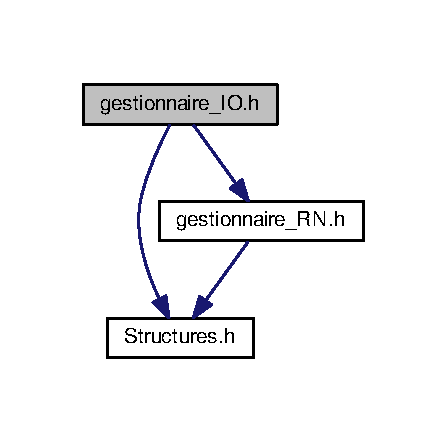
\includegraphics[width=215pt]{gestionnaire__IO_8h__incl}
\end{center}
\end{figure}
Ce graphe montre quels fichiers incluent directement ou indirectement ce fichier \+:
\nopagebreak
\begin{figure}[H]
\begin{center}
\leavevmode
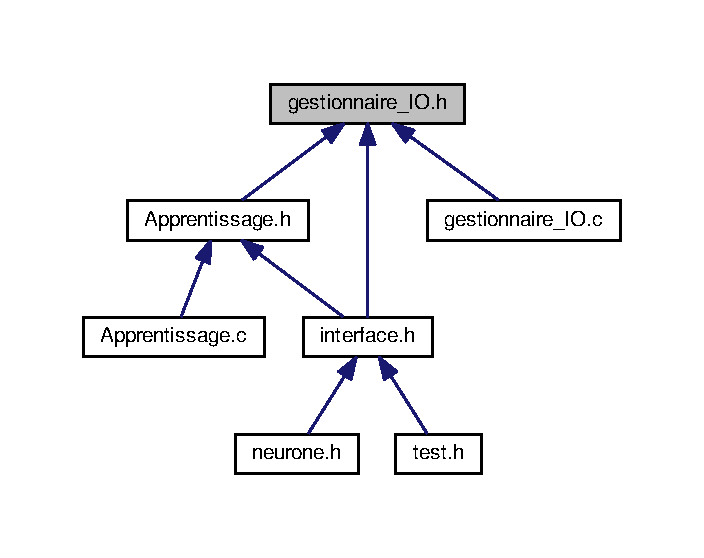
\includegraphics[width=338pt]{gestionnaire__IO_8h__dep__incl}
\end{center}
\end{figure}
\subsection*{Fonctions}
\begin{DoxyCompactItemize}
\item 
\hyperlink{structImage}{Image} $\ast$ \hyperlink{gestionnaire__IO_8h_a219dfd2654f71f643db4d1a5c4c967e4}{Charger\+Bmp} (const char $\ast$fichier, int, int)
\begin{DoxyCompactList}\small\item\em On lis une image de format bmp et on l\textquotesingle{}enregistre dans la structure \hyperlink{structImage}{Image}. \end{DoxyCompactList}\item 
\hyperlink{structImage}{Image} $\ast$ {\bfseries Charger\+Mnist} (const char $\ast$fichier, int, int)\hypertarget{gestionnaire__IO_8h_a1b66f77536ba38756233bc9d1ce332bc}{}\label{gestionnaire__IO_8h_a1b66f77536ba38756233bc9d1ce332bc}

\item 
int {\bfseries Sauver} (\hyperlink{structImage}{Image} $\ast$, const char $\ast$fichier)\hypertarget{gestionnaire__IO_8h_af9f311b71088ee8e148cedea26b57446}{}\label{gestionnaire__IO_8h_af9f311b71088ee8e148cedea26b57446}

\item 
\hyperlink{structImage}{Image} $\ast$ {\bfseries Nouvelle\+Image} (int w, int h)\hypertarget{gestionnaire__IO_8h_ac91839d8b84692804f4b60afe1bb216f}{}\label{gestionnaire__IO_8h_ac91839d8b84692804f4b60afe1bb216f}

\item 
\hyperlink{structImage}{Image} $\ast$ {\bfseries Copie\+Image} (\hyperlink{structImage}{Image} $\ast$)\hypertarget{gestionnaire__IO_8h_ae24d063d2a54338c50361d9637471403}{}\label{gestionnaire__IO_8h_ae24d063d2a54338c50361d9637471403}

\item 
void {\bfseries Set\+Pixel} (\hyperlink{structImage}{Image} $\ast$, int i, int j, \hyperlink{structPixel}{Pixel} p)\hypertarget{gestionnaire__IO_8h_ab1f4e65d86624d222de7abd901eccf53}{}\label{gestionnaire__IO_8h_ab1f4e65d86624d222de7abd901eccf53}

\item 
\hyperlink{structPixel}{Pixel} {\bfseries Get\+Pixel} (\hyperlink{structImage}{Image} $\ast$, int i, int j)\hypertarget{gestionnaire__IO_8h_a74daa7c07ebad562a56512b70cd99773}{}\label{gestionnaire__IO_8h_a74daa7c07ebad562a56512b70cd99773}

\item 
void {\bfseries Del\+Image} (\hyperlink{structImage}{Image} $\ast$)\hypertarget{gestionnaire__IO_8h_a30120c639290b6ab167c09ee75f23b5a}{}\label{gestionnaire__IO_8h_a30120c639290b6ab167c09ee75f23b5a}

\item 
char $\ast$ {\bfseries Charger\+Etiquette\+M\+N\+I\+ST} (const char $\ast$path)\hypertarget{gestionnaire__IO_8h_ad75487d79bfcd9c86941964341b27ed4}{}\label{gestionnaire__IO_8h_ad75487d79bfcd9c86941964341b27ed4}

\item 
\hyperlink{structApprentissage}{App} $\ast$ {\bfseries Chargement\+Couple\+Att\+In} (char $\ast$repertoire\+\_\+app, int w\+\_\+max, int h\+\_\+max)\hypertarget{gestionnaire__IO_8h_af173f0494a794123f2c65871af91ef8b}{}\label{gestionnaire__IO_8h_af173f0494a794123f2c65871af91ef8b}

\item 
\hyperlink{structINFO__RN}{I\+N\+F\+O\+\_\+\+RN} $\ast$ {\bfseries Charger\+Info} ()\hypertarget{gestionnaire__IO_8h_a343472a40d9ee1ed25bb7caf22be1b8f}{}\label{gestionnaire__IO_8h_a343472a40d9ee1ed25bb7caf22be1b8f}

\item 
\hyperlink{structRN}{RN} $\ast$ {\bfseries Charger\+RN} (\hyperlink{structINFO__RN}{I\+N\+F\+O\+\_\+\+RN} $\ast$info)\hypertarget{gestionnaire__IO_8h_af2e5b9ad00cab116ec82a35aa1e1c7f0}{}\label{gestionnaire__IO_8h_af2e5b9ad00cab116ec82a35aa1e1c7f0}

\item 
void {\bfseries Save\+RN} (\hyperlink{structRN}{RN})\hypertarget{gestionnaire__IO_8h_a6a8ff4d9f4c8307e35f700bd10cda07f}{}\label{gestionnaire__IO_8h_a6a8ff4d9f4c8307e35f700bd10cda07f}

\end{DoxyCompactItemize}


\subsection{Description détaillée}
Gestionnaire d\textquotesingle{}entrées sorties. 

\begin{DoxyAuthor}{Auteur}
P\+E\+P\+IN Thibaut 

R\+E\+Z\+G\+UI Soumia 

S\+L\+I\+M\+A\+NI Arezki 

S\+E\+L\+A\+Q\+U\+ET Severine 

S\+Z\+U\+L\+EK Isaac 

M\+O\+N\+T\+I\+G\+N\+ET Anthony
\end{DoxyAuthor}
Ce module s\textquotesingle{}occupe de lire , charger et sauvegarder les données. 

\subsection{Documentation des fonctions}
\index{gestionnaire\+\_\+\+I\+O.\+h@{gestionnaire\+\_\+\+I\+O.\+h}!Charger\+Bmp@{Charger\+Bmp}}
\index{Charger\+Bmp@{Charger\+Bmp}!gestionnaire\+\_\+\+I\+O.\+h@{gestionnaire\+\_\+\+I\+O.\+h}}
\subsubsection[{\texorpdfstring{Charger\+Bmp(const char $\ast$fichier, int, int)}{ChargerBmp(const char *fichier, int, int)}}]{\setlength{\rightskip}{0pt plus 5cm}{\bf Image}$\ast$ Charger\+Bmp (
\begin{DoxyParamCaption}
\item[{const char $\ast$}]{fichier, }
\item[{int}]{w\+\_\+max, }
\item[{int}]{h\+\_\+max}
\end{DoxyParamCaption}
)}\hypertarget{gestionnaire__IO_8h_a219dfd2654f71f643db4d1a5c4c967e4}{}\label{gestionnaire__IO_8h_a219dfd2654f71f643db4d1a5c4c967e4}


On lis une image de format bmp et on l\textquotesingle{}enregistre dans la structure \hyperlink{structImage}{Image}. 


\begin{DoxyParams}{Paramètres}
{\em fichier} & Chemin absolue de l\textquotesingle{}image à charger. \\
\hline
{\em } & \\
\hline
\end{DoxyParams}

\hypertarget{gestionnaire__RN_8c}{}\section{Référence du fichier gestionnaire\+\_\+\+R\+N.\+c}
\label{gestionnaire__RN_8c}\index{gestionnaire\+\_\+\+R\+N.\+c@{gestionnaire\+\_\+\+R\+N.\+c}}


Code de la partie propagation ainsi que toutes les fonctions necessaire a celle ci.  


{\ttfamily \#include $<$math.\+h$>$}\\*
{\ttfamily \#include \char`\"{}gestionnaire\+\_\+\+R\+N.\+h\char`\"{}}\\*
{\ttfamily \#include $<$string.\+h$>$}\\*
{\ttfamily \#include $<$stdlib.\+h$>$}\\*
{\ttfamily \#include $<$stdio.\+h$>$}\\*
{\ttfamily \#include $<$time.\+h$>$}\\*
Graphe des dépendances par inclusion de gestionnaire\+\_\+\+R\+N.\+c\+:
\nopagebreak
\begin{figure}[H]
\begin{center}
\leavevmode
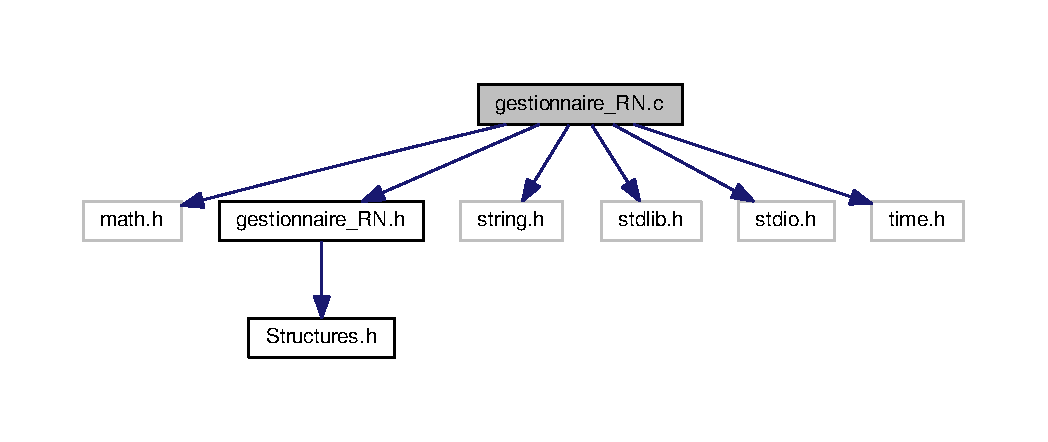
\includegraphics[width=350pt]{gestionnaire__RN_8c__incl}
\end{center}
\end{figure}
\subsection*{Fonctions}
\begin{DoxyCompactItemize}
\item 
void \hyperlink{gestionnaire__RN_8c_a575950fbd65a265a39f7738a7afc6132}{Multiplication\+Matrice\+Vecteur} (float $\ast$$\ast$in\+\_\+M, float $\ast$in\+\_\+V, float $\ast$out, int taille\+\_\+\+M1, int taille\+\_\+\+M3)
\begin{DoxyCompactList}\small\item\em multiplie une matrice avec un vecteur \end{DoxyCompactList}\item 
void \hyperlink{gestionnaire__RN_8c_a658cb025d40aad873b47a60d92409788}{Addition\+Vecteur\+Vecteur} (float $\ast$in\+\_\+\+V1, float $\ast$in\+\_\+\+V2, float $\ast$out, int taille)
\begin{DoxyCompactList}\small\item\em additionne deux vecteur \end{DoxyCompactList}\item 
void \hyperlink{gestionnaire__RN_8c_a88161240b8b73cd76cb6c099c5016722}{SigmoideV} (float $\ast$in\+\_\+V, float $\ast$out, int taille)
\begin{DoxyCompactList}\small\item\em calcule le résulta de la fonction sigmoide sur chacun des éléments du vecteur d\textquotesingle{}entrée \end{DoxyCompactList}\item 
float \hyperlink{gestionnaire__RN_8c_a9437015febf55efc8dd7038bf5b923eb}{Sigmoide} (float in)
\begin{DoxyCompactList}\small\item\em passe un nombre dans la fonction sigmoide \end{DoxyCompactList}\item 
\hyperlink{structRN}{RN} $\ast$ \hyperlink{gestionnaire__RN_8c_a950d3ef952b3ba0129b5b68e1a11ea45}{initialisation} (\hyperlink{structINFO__RN}{I\+N\+F\+O\+\_\+\+RN} $\ast$info)
\begin{DoxyCompactList}\small\item\em initialise un réseau de neurone a partir d\textquotesingle{}une structure \hyperlink{structINFO__RN}{I\+N\+F\+O\+\_\+\+RN} \end{DoxyCompactList}\item 
void \hyperlink{gestionnaire__RN_8c_aec2e4ad8ae3d56448565c8057ad15c8f}{Remplissage} (\hyperlink{structRN}{RN} rn)
\begin{DoxyCompactList}\small\item\em met des valeurs aléatoire dans les poids et les biais du réseau de neurone \end{DoxyCompactList}\item 
void \hyperlink{gestionnaire__RN_8c_a296597a276e828328d98e3262070628d}{Ajout\+\_\+couche\+\_\+\+Fin} (\hyperlink{structRN}{RN} $\ast$rn, int taille)
\begin{DoxyCompactList}\small\item\em ajoute une couche au réseau de neurone \end{DoxyCompactList}\item 
void \hyperlink{gestionnaire__RN_8c_a46cf75e38a207cde73b63419744e51e0}{Ajout\+Premiere\+Couche} (\hyperlink{structRN}{RN} $\ast$rn, int taille)
\begin{DoxyCompactList}\small\item\em ajoute la premiere couche d\textquotesingle{}un réseau de neurone \end{DoxyCompactList}\item 
void \hyperlink{gestionnaire__RN_8c_ac8d3388e91ece80910d34dbee00af979}{Propagation} (\hyperlink{structImage}{Image} $\ast$im, \hyperlink{structRN}{RN} rn)
\begin{DoxyCompactList}\small\item\em effectue l\textquotesingle{}algorithme de propagation \end{DoxyCompactList}\item 
char $\ast$$\ast$ \hyperlink{gestionnaire__RN_8c_a8021aaff66ae4a05e06737e94fec55de}{Reconnaissance} (\hyperlink{structRN}{RN} rn)
\begin{DoxyCompactList}\small\item\em trouve les trois neurone de la couche de fin ayant la plus grande activation et renvois leur étiquette. \end{DoxyCompactList}\item 
void \hyperlink{gestionnaire__RN_8c_a196954462b6e56784bd7cd9f0e9e5c2e}{liberer\+RN} (\hyperlink{structRN}{RN} $\ast$rn)
\begin{DoxyCompactList}\small\item\em libere la mémoire occupée par un réseau de neurone \end{DoxyCompactList}\end{DoxyCompactItemize}


\subsection{Description détaillée}
Code de la partie propagation ainsi que toutes les fonctions necessaire a celle ci. 

\begin{DoxyAuthor}{Auteur}
P\+E\+P\+IN Thibaut 

R\+E\+Z\+G\+UI Soumia 

S\+L\+I\+M\+A\+NI Arezki 

S\+E\+L\+A\+Q\+U\+ET Severine 

S\+Z\+U\+L\+EK Isaac 

M\+O\+N\+T\+I\+G\+N\+ET Anthony 
\end{DoxyAuthor}


\subsection{Documentation des fonctions}
\index{gestionnaire\+\_\+\+R\+N.\+c@{gestionnaire\+\_\+\+R\+N.\+c}!Addition\+Vecteur\+Vecteur@{Addition\+Vecteur\+Vecteur}}
\index{Addition\+Vecteur\+Vecteur@{Addition\+Vecteur\+Vecteur}!gestionnaire\+\_\+\+R\+N.\+c@{gestionnaire\+\_\+\+R\+N.\+c}}
\subsubsection[{\texorpdfstring{Addition\+Vecteur\+Vecteur(float $\ast$in\+\_\+\+V1, float $\ast$in\+\_\+\+V2, float $\ast$out, int taille)}{AdditionVecteurVecteur(float *in_V1, float *in_V2, float *out, int taille)}}]{\setlength{\rightskip}{0pt plus 5cm}void Addition\+Vecteur\+Vecteur (
\begin{DoxyParamCaption}
\item[{float $\ast$}]{in\+\_\+\+V1, }
\item[{float $\ast$}]{in\+\_\+\+V2, }
\item[{float $\ast$}]{out, }
\item[{int}]{taille}
\end{DoxyParamCaption}
)}\hypertarget{gestionnaire__RN_8c_a658cb025d40aad873b47a60d92409788}{}\label{gestionnaire__RN_8c_a658cb025d40aad873b47a60d92409788}


additionne deux vecteur 


\begin{DoxyParams}{Paramètres}
{\em in\+\_\+\+V1} & premier vecteur de l\textquotesingle{}opération \\
\hline
{\em in\+\_\+\+V2} & deuxieme vecteur de l\textquotesingle{}opération \\
\hline
{\em out} & vecteur ou est stocké le résultat \\
\hline
{\em taille} & taille des vecteurs \\
\hline
\end{DoxyParams}
\index{gestionnaire\+\_\+\+R\+N.\+c@{gestionnaire\+\_\+\+R\+N.\+c}!Ajout\+\_\+couche\+\_\+\+Fin@{Ajout\+\_\+couche\+\_\+\+Fin}}
\index{Ajout\+\_\+couche\+\_\+\+Fin@{Ajout\+\_\+couche\+\_\+\+Fin}!gestionnaire\+\_\+\+R\+N.\+c@{gestionnaire\+\_\+\+R\+N.\+c}}
\subsubsection[{\texorpdfstring{Ajout\+\_\+couche\+\_\+\+Fin(\+R\+N $\ast$rn, int taille)}{Ajout_couche_Fin(RN *rn, int taille)}}]{\setlength{\rightskip}{0pt plus 5cm}void Ajout\+\_\+couche\+\_\+\+Fin (
\begin{DoxyParamCaption}
\item[{{\bf RN} $\ast$}]{rn, }
\item[{int}]{taille}
\end{DoxyParamCaption}
)}\hypertarget{gestionnaire__RN_8c_a296597a276e828328d98e3262070628d}{}\label{gestionnaire__RN_8c_a296597a276e828328d98e3262070628d}


ajoute une couche au réseau de neurone 


\begin{DoxyParams}{Paramètres}
{\em rn} & réseau ou rajouter une couche \\
\hline
{\em taille} & nombre de neurones de la couche a rajouter \\
\hline
\end{DoxyParams}
\index{gestionnaire\+\_\+\+R\+N.\+c@{gestionnaire\+\_\+\+R\+N.\+c}!Ajout\+Premiere\+Couche@{Ajout\+Premiere\+Couche}}
\index{Ajout\+Premiere\+Couche@{Ajout\+Premiere\+Couche}!gestionnaire\+\_\+\+R\+N.\+c@{gestionnaire\+\_\+\+R\+N.\+c}}
\subsubsection[{\texorpdfstring{Ajout\+Premiere\+Couche(\+R\+N $\ast$rn, int taille)}{AjoutPremiereCouche(RN *rn, int taille)}}]{\setlength{\rightskip}{0pt plus 5cm}void Ajout\+Premiere\+Couche (
\begin{DoxyParamCaption}
\item[{{\bf RN} $\ast$}]{rn, }
\item[{int}]{taille}
\end{DoxyParamCaption}
)}\hypertarget{gestionnaire__RN_8c_a46cf75e38a207cde73b63419744e51e0}{}\label{gestionnaire__RN_8c_a46cf75e38a207cde73b63419744e51e0}


ajoute la premiere couche d\textquotesingle{}un réseau de neurone 


\begin{DoxyParams}{Paramètres}
{\em rn} & réseau ou rajouter la couche \\
\hline
{\em taille} & nombre de neurones de la couche a rajouter \\
\hline
\end{DoxyParams}
\index{gestionnaire\+\_\+\+R\+N.\+c@{gestionnaire\+\_\+\+R\+N.\+c}!initialisation@{initialisation}}
\index{initialisation@{initialisation}!gestionnaire\+\_\+\+R\+N.\+c@{gestionnaire\+\_\+\+R\+N.\+c}}
\subsubsection[{\texorpdfstring{initialisation(\+I\+N\+F\+O\+\_\+\+R\+N $\ast$info)}{initialisation(INFO_RN *info)}}]{\setlength{\rightskip}{0pt plus 5cm}{\bf RN} $\ast$ initialisation (
\begin{DoxyParamCaption}
\item[{{\bf I\+N\+F\+O\+\_\+\+RN} $\ast$}]{info}
\end{DoxyParamCaption}
)}\hypertarget{gestionnaire__RN_8c_a950d3ef952b3ba0129b5b68e1a11ea45}{}\label{gestionnaire__RN_8c_a950d3ef952b3ba0129b5b68e1a11ea45}


initialise un réseau de neurone a partir d\textquotesingle{}une structure \hyperlink{structINFO__RN}{I\+N\+F\+O\+\_\+\+RN} 


\begin{DoxyParams}{Paramètres}
{\em info} & structure contenant diverse information sur le réseau de neurone a initialiser \\
\hline
\end{DoxyParams}
\begin{DoxyReturn}{Renvoie}
le réseau de neurone initialisé 
\end{DoxyReturn}
\index{gestionnaire\+\_\+\+R\+N.\+c@{gestionnaire\+\_\+\+R\+N.\+c}!liberer\+RN@{liberer\+RN}}
\index{liberer\+RN@{liberer\+RN}!gestionnaire\+\_\+\+R\+N.\+c@{gestionnaire\+\_\+\+R\+N.\+c}}
\subsubsection[{\texorpdfstring{liberer\+R\+N(\+R\+N $\ast$rn)}{libererRN(RN *rn)}}]{\setlength{\rightskip}{0pt plus 5cm}void liberer\+RN (
\begin{DoxyParamCaption}
\item[{{\bf RN} $\ast$}]{rn}
\end{DoxyParamCaption}
)}\hypertarget{gestionnaire__RN_8c_a196954462b6e56784bd7cd9f0e9e5c2e}{}\label{gestionnaire__RN_8c_a196954462b6e56784bd7cd9f0e9e5c2e}


libere la mémoire occupée par un réseau de neurone 


\begin{DoxyParams}{Paramètres}
{\em rn} & réseau de neurone a liberer \\
\hline
\end{DoxyParams}
\index{gestionnaire\+\_\+\+R\+N.\+c@{gestionnaire\+\_\+\+R\+N.\+c}!Multiplication\+Matrice\+Vecteur@{Multiplication\+Matrice\+Vecteur}}
\index{Multiplication\+Matrice\+Vecteur@{Multiplication\+Matrice\+Vecteur}!gestionnaire\+\_\+\+R\+N.\+c@{gestionnaire\+\_\+\+R\+N.\+c}}
\subsubsection[{\texorpdfstring{Multiplication\+Matrice\+Vecteur(float $\ast$$\ast$in\+\_\+\+M, float $\ast$in\+\_\+\+V, float $\ast$out, int taille\+\_\+\+M1, int taille\+\_\+\+M3)}{MultiplicationMatriceVecteur(float **in_M, float *in_V, float *out, int taille_M1, int taille_M3)}}]{\setlength{\rightskip}{0pt plus 5cm}void Multiplication\+Matrice\+Vecteur (
\begin{DoxyParamCaption}
\item[{float $\ast$$\ast$}]{in\+\_\+M, }
\item[{float $\ast$}]{in\+\_\+V, }
\item[{float $\ast$}]{out, }
\item[{int}]{taille\+\_\+\+M1, }
\item[{int}]{taille\+\_\+\+M3}
\end{DoxyParamCaption}
)}\hypertarget{gestionnaire__RN_8c_a575950fbd65a265a39f7738a7afc6132}{}\label{gestionnaire__RN_8c_a575950fbd65a265a39f7738a7afc6132}


multiplie une matrice avec un vecteur 


\begin{DoxyParams}{Paramètres}
{\em in\+\_\+M} & matrice de l\textquotesingle{}opération \\
\hline
{\em in\+\_\+V} & vecteur de l\textquotesingle{}opération \\
\hline
{\em out} & vecteur ou est stocké le résultat \\
\hline
{\em taille\+\_\+\+M1} & hauteur de la matrice \\
\hline
{\em taille\+\_\+\+M3} & largeur de la matrice \\
\hline
\end{DoxyParams}
\index{gestionnaire\+\_\+\+R\+N.\+c@{gestionnaire\+\_\+\+R\+N.\+c}!Propagation@{Propagation}}
\index{Propagation@{Propagation}!gestionnaire\+\_\+\+R\+N.\+c@{gestionnaire\+\_\+\+R\+N.\+c}}
\subsubsection[{\texorpdfstring{Propagation(\+Image $\ast$im, R\+N rn)}{Propagation(Image *im, RN rn)}}]{\setlength{\rightskip}{0pt plus 5cm}void Propagation (
\begin{DoxyParamCaption}
\item[{{\bf Image} $\ast$}]{im, }
\item[{{\bf RN}}]{rn}
\end{DoxyParamCaption}
)}\hypertarget{gestionnaire__RN_8c_ac8d3388e91ece80910d34dbee00af979}{}\label{gestionnaire__RN_8c_ac8d3388e91ece80910d34dbee00af979}


effectue l\textquotesingle{}algorithme de propagation 


\begin{DoxyParams}{Paramètres}
{\em im} & l\textquotesingle{}information a propager dans le réseau de neurone \\
\hline
{\em rn} & réseau ou effectuer la ropagation \\
\hline
\end{DoxyParams}
\index{gestionnaire\+\_\+\+R\+N.\+c@{gestionnaire\+\_\+\+R\+N.\+c}!Reconnaissance@{Reconnaissance}}
\index{Reconnaissance@{Reconnaissance}!gestionnaire\+\_\+\+R\+N.\+c@{gestionnaire\+\_\+\+R\+N.\+c}}
\subsubsection[{\texorpdfstring{Reconnaissance(\+R\+N rn)}{Reconnaissance(RN rn)}}]{\setlength{\rightskip}{0pt plus 5cm}char $\ast$$\ast$ Reconnaissance (
\begin{DoxyParamCaption}
\item[{{\bf RN}}]{rn}
\end{DoxyParamCaption}
)}\hypertarget{gestionnaire__RN_8c_a8021aaff66ae4a05e06737e94fec55de}{}\label{gestionnaire__RN_8c_a8021aaff66ae4a05e06737e94fec55de}


trouve les trois neurone de la couche de fin ayant la plus grande activation et renvois leur étiquette. 


\begin{DoxyParams}{Paramètres}
{\em rn} & réseau ous\textquotesingle{}effectue l\textquotesingle{}analyse de la couche de fin \\
\hline
\end{DoxyParams}
\begin{DoxyReturn}{Renvoie}
un tableau de trois chaine de caractères contenant les étiquette des trois neurone de la couche de fin ayant la plus grande activation. 
\end{DoxyReturn}
\index{gestionnaire\+\_\+\+R\+N.\+c@{gestionnaire\+\_\+\+R\+N.\+c}!Remplissage@{Remplissage}}
\index{Remplissage@{Remplissage}!gestionnaire\+\_\+\+R\+N.\+c@{gestionnaire\+\_\+\+R\+N.\+c}}
\subsubsection[{\texorpdfstring{Remplissage(\+R\+N rn)}{Remplissage(RN rn)}}]{\setlength{\rightskip}{0pt plus 5cm}void Remplissage (
\begin{DoxyParamCaption}
\item[{{\bf RN}}]{rn}
\end{DoxyParamCaption}
)}\hypertarget{gestionnaire__RN_8c_aec2e4ad8ae3d56448565c8057ad15c8f}{}\label{gestionnaire__RN_8c_aec2e4ad8ae3d56448565c8057ad15c8f}


met des valeurs aléatoire dans les poids et les biais du réseau de neurone 


\begin{DoxyParams}{Paramètres}
{\em rn} & réseau de neurone a remplir \\
\hline
\end{DoxyParams}
\index{gestionnaire\+\_\+\+R\+N.\+c@{gestionnaire\+\_\+\+R\+N.\+c}!Sigmoide@{Sigmoide}}
\index{Sigmoide@{Sigmoide}!gestionnaire\+\_\+\+R\+N.\+c@{gestionnaire\+\_\+\+R\+N.\+c}}
\subsubsection[{\texorpdfstring{Sigmoide(float in)}{Sigmoide(float in)}}]{\setlength{\rightskip}{0pt plus 5cm}float Sigmoide (
\begin{DoxyParamCaption}
\item[{float}]{in}
\end{DoxyParamCaption}
)}\hypertarget{gestionnaire__RN_8c_a9437015febf55efc8dd7038bf5b923eb}{}\label{gestionnaire__RN_8c_a9437015febf55efc8dd7038bf5b923eb}


passe un nombre dans la fonction sigmoide 


\begin{DoxyParams}{Paramètres}
{\em in} & nombre a passer dans la sigmoide \\
\hline
\end{DoxyParams}
\begin{DoxyReturn}{Renvoie}
valeur de retour de la fonction sigmoide 
\end{DoxyReturn}
\index{gestionnaire\+\_\+\+R\+N.\+c@{gestionnaire\+\_\+\+R\+N.\+c}!SigmoideV@{SigmoideV}}
\index{SigmoideV@{SigmoideV}!gestionnaire\+\_\+\+R\+N.\+c@{gestionnaire\+\_\+\+R\+N.\+c}}
\subsubsection[{\texorpdfstring{Sigmoide\+V(float $\ast$in\+\_\+\+V, float $\ast$out, int taille)}{SigmoideV(float *in_V, float *out, int taille)}}]{\setlength{\rightskip}{0pt plus 5cm}void SigmoideV (
\begin{DoxyParamCaption}
\item[{float $\ast$}]{in\+\_\+V, }
\item[{float $\ast$}]{out, }
\item[{int}]{taille}
\end{DoxyParamCaption}
)}\hypertarget{gestionnaire__RN_8c_a88161240b8b73cd76cb6c099c5016722}{}\label{gestionnaire__RN_8c_a88161240b8b73cd76cb6c099c5016722}


calcule le résulta de la fonction sigmoide sur chacun des éléments du vecteur d\textquotesingle{}entrée 


\begin{DoxyParams}{Paramètres}
{\em in\+\_\+V} & vecteur contenant les valeurs \\
\hline
{\em out} & vecteur ou est stocké le résultat \\
\hline
{\em taille} & taille du vecteur d\textquotesingle{}entrée \\
\hline
\end{DoxyParams}

\hypertarget{interface_8h}{}\section{Référence du fichier interface.\+h}
\label{interface_8h}\index{interface.\+h@{interface.\+h}}


Interface du programme.  


{\ttfamily \#include \char`\"{}gestionnaire\+\_\+\+R\+N.\+h\char`\"{}}\\*
{\ttfamily \#include \char`\"{}Apprentissage.\+h\char`\"{}}\\*
{\ttfamily \#include \char`\"{}gestionnaire\+\_\+\+I\+O.\+h\char`\"{}}\\*
{\ttfamily \#include \char`\"{}Structures.\+h\char`\"{}}\\*
{\ttfamily \#include $<$stdio.\+h$>$}\\*
{\ttfamily \#include $<$stdlib.\+h$>$}\\*
{\ttfamily \#include $<$string.\+h$>$}\\*
{\ttfamily \#include $<$assert.\+h$>$}\\*
{\ttfamily \#include $<$time.\+h$>$}\\*
{\ttfamily \#include $<$pthread.\+h$>$}\\*
{\ttfamily \#include $<$sys/types.\+h$>$}\\*
{\ttfamily \#include $<$dirent.\+h$>$}\\*
{\ttfamily \#include $<$sys/dir.\+h$>$}\\*
{\ttfamily \#include $<$errno.\+h$>$}\\*
{\ttfamily \#include $<$sys/stat.\+h$>$}\\*
{\ttfamily \#include $<$gtk/gtk.\+h$>$}\\*
Graphe des dépendances par inclusion de interface.\+h\+:
\nopagebreak
\begin{figure}[H]
\begin{center}
\leavevmode
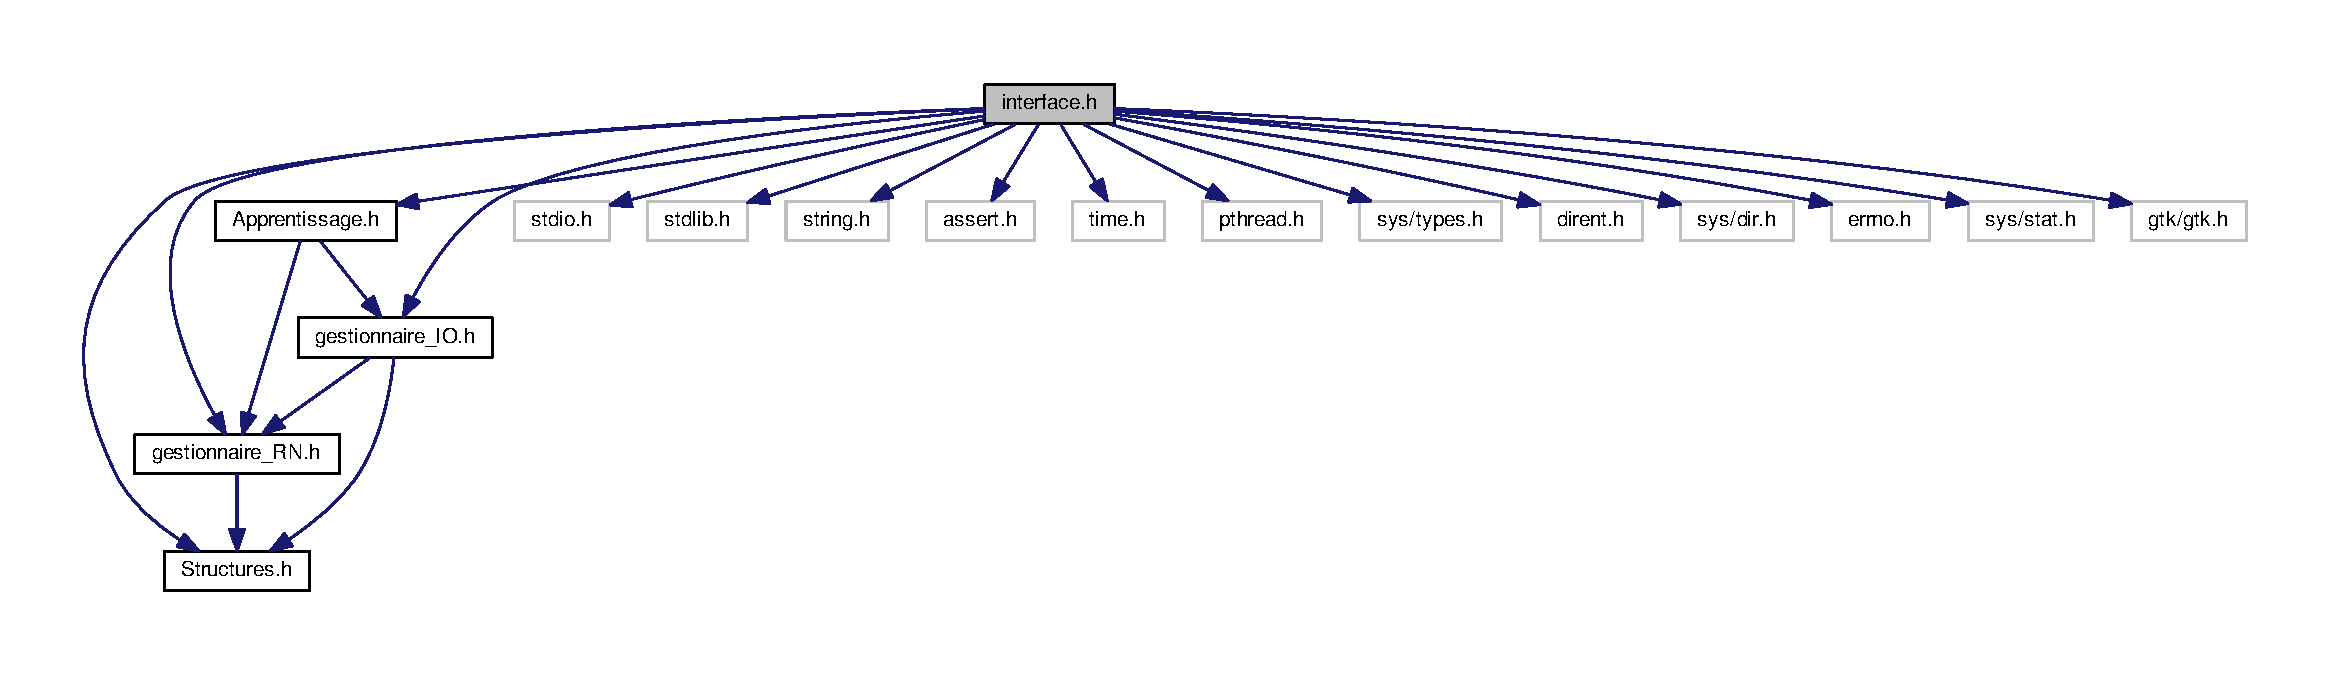
\includegraphics[width=350pt]{interface_8h__incl}
\end{center}
\end{figure}
Ce graphe montre quels fichiers incluent directement ou indirectement ce fichier \+:
\nopagebreak
\begin{figure}[H]
\begin{center}
\leavevmode
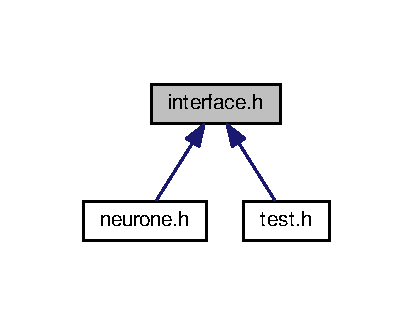
\includegraphics[width=198pt]{interface_8h__dep__incl}
\end{center}
\end{figure}
\subsection*{Classes}
\begin{DoxyCompactItemize}
\item 
struct \hyperlink{structINFO__FENETRE}{I\+N\+F\+O\+\_\+\+F\+E\+N\+E\+T\+RE}
\begin{DoxyCompactList}\small\item\em Information circulant entre les fonctions. \end{DoxyCompactList}\end{DoxyCompactItemize}
\subsection*{Définitions de type}
\begin{DoxyCompactItemize}
\item 
typedef struct \hyperlink{structINFO__FENETRE}{I\+N\+F\+O\+\_\+\+F\+E\+N\+E\+T\+RE} {\bfseries I\+N\+F\+O\+\_\+\+F\+E\+N\+E\+T\+RE}\hypertarget{interface_8h_aead7bcd5aa775cd161b684815cef6e5a}{}\label{interface_8h_aead7bcd5aa775cd161b684815cef6e5a}

\end{DoxyCompactItemize}
\subsection*{Fonctions}
\begin{DoxyCompactItemize}
\item 
int \hyperlink{interface_8h_a1157bf477c8e67641948cb31de95754e}{nombre\+Reseau} ()
\begin{DoxyCompactList}\small\item\em Nombre de Réseaux de neurones existant. \end{DoxyCompactList}\item 
void \hyperlink{interface_8h_a08aaf6738ef116b20809fd4c3af451ea}{vider\+Container} (Gtk\+Widget $\ast$data)
\begin{DoxyCompactList}\small\item\em Vider le contenu de la fenetre. \end{DoxyCompactList}\item 
void \hyperlink{interface_8h_ab377f1cf5a8abbe888b67875fe00e732}{retour\+Accueille} (Gtk\+Widget $\ast$widget, gpointer data)
\begin{DoxyCompactList}\small\item\em Retourner a la page d\textquotesingle{}accueille. \end{DoxyCompactList}\item 
void \hyperlink{interface_8h_a4aaaee29e9c54955715a9de0be73563d}{select\+Reseau} (Gtk\+Widget $\ast$widget, gpointer data)
\begin{DoxyCompactList}\small\item\em Selection d\textquotesingle{}un reseau de neurone. \end{DoxyCompactList}\item 
void \hyperlink{interface_8h_aed9f60cdb4aaeaf5500cd93cce7a1b6d}{traitement} (Gtk\+Widget $\ast$widget, gpointer data)
\begin{DoxyCompactList}\small\item\em Lance le traitement d\textquotesingle{}une image. \end{DoxyCompactList}\item 
void \hyperlink{interface_8h_af336de7bd25d6d5909517f909a171b37}{lancer\+Apprentissage} (Gtk\+Widget $\ast$widget, gpointer data)
\begin{DoxyCompactList}\small\item\em Lancer l\textquotesingle{}apprentissage du réseau de neurones. \end{DoxyCompactList}\item 
void $\ast$ \hyperlink{interface_8h_a92b101b532f98164c1f609dec68afe00}{fct\+Thread\+App} (void $\ast$arg)
\begin{DoxyCompactList}\small\item\em Fonction appeler par le thread qui fait l\textquotesingle{}apprentissage du reseau de neurone. \end{DoxyCompactList}\item 
void \hyperlink{interface_8h_ae0a8eb01de87316e3486addd8b177515}{matrice} (Gtk\+Widget $\ast$widget, gpointer data)
\begin{DoxyCompactList}\small\item\em Affichage de la matrice des poid du reseau de neurones. \end{DoxyCompactList}\item 
void \hyperlink{interface_8h_af05673f8ea4045e8dc3eacdbf80f3eb6}{resultat\+Traitement} (Gtk\+Widget $\ast$widget, gpointer data)
\begin{DoxyCompactList}\small\item\em Affiche le résultat du traitement d\textquotesingle{}une image. \end{DoxyCompactList}\item 
void \hyperlink{interface_8h_ab697526e222972bbbee4f4429daf38cc}{page\+\_\+principale} (\hyperlink{structINFO__FENETRE}{I\+N\+F\+O\+\_\+\+F\+E\+N\+E\+T\+RE} $\ast$fenetre)
\begin{DoxyCompactList}\small\item\em Page d\textquotesingle{}accueille du programme. \end{DoxyCompactList}\item 
void \hyperlink{interface_8h_aa7658136cafa28ec67a73274f310a7b4}{creer\+\_\+file\+\_\+selection} ()
\begin{DoxyCompactList}\small\item\em Selection d\textquotesingle{}un fichier a analyser dans traitement. \end{DoxyCompactList}\item 
void \hyperlink{interface_8h_aeb7db74660ad3d28b2b68874d30d9316}{creer\+\_\+folder\+\_\+selection} (Gtk\+Button $\ast$button, gpointer data)
\begin{DoxyCompactList}\small\item\em Selection du dossier ou ce trouverons les données pour l\textquotesingle{}apprentissage. \end{DoxyCompactList}\item 
void \hyperlink{interface_8h_a15cf03bc8aef74929090ec43f9dcd1d6}{creation} (Gtk\+Widget $\ast$widget, gpointer data)
\begin{DoxyCompactList}\small\item\em Interface de creation d\textquotesingle{}un reseau de neurones. \end{DoxyCompactList}\item 
void {\bfseries creation\+RN} (Gtk\+Widget $\ast$widget, gpointer data)\hypertarget{interface_8h_afb7b9f7924beb4a920220bb2d9a13245}{}\label{interface_8h_afb7b9f7924beb4a920220bb2d9a13245}

\item 
void \hyperlink{interface_8h_aea683c3c50c9b394b3145ffa90bac3a5}{quitter} (Gtk\+Widget $\ast$widget, gpointer data)
\begin{DoxyCompactList}\small\item\em Lorsque l\textquotesingle{}on quitte la fenetre. \end{DoxyCompactList}\item 
void \hyperlink{interface_8h_a892c9f29f308cd1e9db0ec363ebc2861}{afficher\+Interface} ()
\begin{DoxyCompactList}\small\item\em Contenant toute l\textquotesingle{}interface et les fonction. \end{DoxyCompactList}\end{DoxyCompactItemize}


\subsection{Description détaillée}
Interface du programme. 

\begin{DoxyAuthor}{Auteur}
P\+E\+P\+IN Thibaut 

R\+E\+Z\+G\+UI Soumia 

S\+L\+I\+M\+A\+NI Arezki 

S\+E\+L\+A\+Q\+U\+ET Severine 

S\+Z\+U\+L\+EK Isaac 

M\+O\+N\+T\+I\+G\+N\+ET Anthony
\end{DoxyAuthor}
Interface du programme de reconnaissance d\textquotesingle{}image. 

\subsection{Documentation des fonctions}
\index{interface.\+h@{interface.\+h}!afficher\+Interface@{afficher\+Interface}}
\index{afficher\+Interface@{afficher\+Interface}!interface.\+h@{interface.\+h}}
\subsubsection[{\texorpdfstring{afficher\+Interface()}{afficherInterface()}}]{\setlength{\rightskip}{0pt plus 5cm}void afficher\+Interface (
\begin{DoxyParamCaption}
{}
\end{DoxyParamCaption}
)}\hypertarget{interface_8h_a892c9f29f308cd1e9db0ec363ebc2861}{}\label{interface_8h_a892c9f29f308cd1e9db0ec363ebc2861}


Contenant toute l\textquotesingle{}interface et les fonction. 

\index{interface.\+h@{interface.\+h}!creation@{creation}}
\index{creation@{creation}!interface.\+h@{interface.\+h}}
\subsubsection[{\texorpdfstring{creation(\+Gtk\+Widget $\ast$widget, gpointer data)}{creation(GtkWidget *widget, gpointer data)}}]{\setlength{\rightskip}{0pt plus 5cm}void creation (
\begin{DoxyParamCaption}
\item[{Gtk\+Widget $\ast$}]{widget, }
\item[{gpointer}]{data}
\end{DoxyParamCaption}
)}\hypertarget{interface_8h_a15cf03bc8aef74929090ec43f9dcd1d6}{}\label{interface_8h_a15cf03bc8aef74929090ec43f9dcd1d6}


Interface de creation d\textquotesingle{}un reseau de neurones. 

Recuperation des données et sauvegarde du réseau de neurones.


\begin{DoxyParams}{Paramètres}
{\em widget} & Le widget qui est associer a la fonction. \\
\hline
{\em data} & Pour le passage de la structure \hyperlink{structINFO__FENETRE}{I\+N\+F\+O\+\_\+\+F\+E\+N\+E\+T\+RE}. \\
\hline
\end{DoxyParams}
\index{interface.\+h@{interface.\+h}!creer\+\_\+file\+\_\+selection@{creer\+\_\+file\+\_\+selection}}
\index{creer\+\_\+file\+\_\+selection@{creer\+\_\+file\+\_\+selection}!interface.\+h@{interface.\+h}}
\subsubsection[{\texorpdfstring{creer\+\_\+file\+\_\+selection()}{creer_file_selection()}}]{\setlength{\rightskip}{0pt plus 5cm}void creer\+\_\+file\+\_\+selection (
\begin{DoxyParamCaption}
{}
\end{DoxyParamCaption}
)}\hypertarget{interface_8h_aa7658136cafa28ec67a73274f310a7b4}{}\label{interface_8h_aa7658136cafa28ec67a73274f310a7b4}


Selection d\textquotesingle{}un fichier a analyser dans traitement. 

\index{interface.\+h@{interface.\+h}!creer\+\_\+folder\+\_\+selection@{creer\+\_\+folder\+\_\+selection}}
\index{creer\+\_\+folder\+\_\+selection@{creer\+\_\+folder\+\_\+selection}!interface.\+h@{interface.\+h}}
\subsubsection[{\texorpdfstring{creer\+\_\+folder\+\_\+selection(\+Gtk\+Button $\ast$button, gpointer data)}{creer_folder_selection(GtkButton *button, gpointer data)}}]{\setlength{\rightskip}{0pt plus 5cm}void creer\+\_\+folder\+\_\+selection (
\begin{DoxyParamCaption}
\item[{Gtk\+Button $\ast$}]{button, }
\item[{gpointer}]{data}
\end{DoxyParamCaption}
)}\hypertarget{interface_8h_aeb7db74660ad3d28b2b68874d30d9316}{}\label{interface_8h_aeb7db74660ad3d28b2b68874d30d9316}


Selection du dossier ou ce trouverons les données pour l\textquotesingle{}apprentissage. 


\begin{DoxyParams}{Paramètres}
{\em widget} & Le widget qui est associer a la fonction. \\
\hline
{\em data} & Pour le passage de la structure \hyperlink{structINFO__FENETRE}{I\+N\+F\+O\+\_\+\+F\+E\+N\+E\+T\+RE}. \\
\hline
\end{DoxyParams}
\index{interface.\+h@{interface.\+h}!fct\+Thread\+App@{fct\+Thread\+App}}
\index{fct\+Thread\+App@{fct\+Thread\+App}!interface.\+h@{interface.\+h}}
\subsubsection[{\texorpdfstring{fct\+Thread\+App(void $\ast$arg)}{fctThreadApp(void *arg)}}]{\setlength{\rightskip}{0pt plus 5cm}void$\ast$ fct\+Thread\+App (
\begin{DoxyParamCaption}
\item[{void $\ast$}]{arg}
\end{DoxyParamCaption}
)}\hypertarget{interface_8h_a92b101b532f98164c1f609dec68afe00}{}\label{interface_8h_a92b101b532f98164c1f609dec68afe00}


Fonction appeler par le thread qui fait l\textquotesingle{}apprentissage du reseau de neurone. 


\begin{DoxyParams}{Paramètres}
{\em arg} & Pour le passage de la structure \hyperlink{structINFO__FENETRE}{I\+N\+F\+O\+\_\+\+F\+E\+N\+E\+T\+RE}. \\
\hline
\end{DoxyParams}
\index{interface.\+h@{interface.\+h}!lancer\+Apprentissage@{lancer\+Apprentissage}}
\index{lancer\+Apprentissage@{lancer\+Apprentissage}!interface.\+h@{interface.\+h}}
\subsubsection[{\texorpdfstring{lancer\+Apprentissage(\+Gtk\+Widget $\ast$widget, gpointer data)}{lancerApprentissage(GtkWidget *widget, gpointer data)}}]{\setlength{\rightskip}{0pt plus 5cm}void lancer\+Apprentissage (
\begin{DoxyParamCaption}
\item[{Gtk\+Widget $\ast$}]{widget, }
\item[{gpointer}]{data}
\end{DoxyParamCaption}
)}\hypertarget{interface_8h_af336de7bd25d6d5909517f909a171b37}{}\label{interface_8h_af336de7bd25d6d5909517f909a171b37}


Lancer l\textquotesingle{}apprentissage du réseau de neurones. 


\begin{DoxyParams}{Paramètres}
{\em widget} & Le widget qui est associer a la fonction. \\
\hline
{\em data} & Pour le passage de la structure \hyperlink{structINFO__FENETRE}{I\+N\+F\+O\+\_\+\+F\+E\+N\+E\+T\+RE}. \\
\hline
\end{DoxyParams}
\index{interface.\+h@{interface.\+h}!matrice@{matrice}}
\index{matrice@{matrice}!interface.\+h@{interface.\+h}}
\subsubsection[{\texorpdfstring{matrice(\+Gtk\+Widget $\ast$widget, gpointer data)}{matrice(GtkWidget *widget, gpointer data)}}]{\setlength{\rightskip}{0pt plus 5cm}void matrice (
\begin{DoxyParamCaption}
\item[{Gtk\+Widget $\ast$}]{widget, }
\item[{gpointer}]{data}
\end{DoxyParamCaption}
)}\hypertarget{interface_8h_ae0a8eb01de87316e3486addd8b177515}{}\label{interface_8h_ae0a8eb01de87316e3486addd8b177515}


Affichage de la matrice des poid du reseau de neurones. 


\begin{DoxyParams}{Paramètres}
{\em widget} & Le widget qui est associer a la fonction. \\
\hline
{\em data} & Pour le passage de la structure \hyperlink{structINFO__FENETRE}{I\+N\+F\+O\+\_\+\+F\+E\+N\+E\+T\+RE}. \\
\hline
\end{DoxyParams}
\index{interface.\+h@{interface.\+h}!nombre\+Reseau@{nombre\+Reseau}}
\index{nombre\+Reseau@{nombre\+Reseau}!interface.\+h@{interface.\+h}}
\subsubsection[{\texorpdfstring{nombre\+Reseau()}{nombreReseau()}}]{\setlength{\rightskip}{0pt plus 5cm}int nombre\+Reseau (
\begin{DoxyParamCaption}
{}
\end{DoxyParamCaption}
)}\hypertarget{interface_8h_a1157bf477c8e67641948cb31de95754e}{}\label{interface_8h_a1157bf477c8e67641948cb31de95754e}


Nombre de Réseaux de neurones existant. 

\begin{DoxyReturn}{Renvoie}
int nombre de Réseau. 
\end{DoxyReturn}
\index{interface.\+h@{interface.\+h}!page\+\_\+principale@{page\+\_\+principale}}
\index{page\+\_\+principale@{page\+\_\+principale}!interface.\+h@{interface.\+h}}
\subsubsection[{\texorpdfstring{page\+\_\+principale(\+I\+N\+F\+O\+\_\+\+F\+E\+N\+E\+T\+R\+E $\ast$fenetre)}{page_principale(INFO_FENETRE *fenetre)}}]{\setlength{\rightskip}{0pt plus 5cm}void page\+\_\+principale (
\begin{DoxyParamCaption}
\item[{{\bf I\+N\+F\+O\+\_\+\+F\+E\+N\+E\+T\+RE} $\ast$}]{fenetre}
\end{DoxyParamCaption}
)}\hypertarget{interface_8h_ab697526e222972bbbee4f4429daf38cc}{}\label{interface_8h_ab697526e222972bbbee4f4429daf38cc}


Page d\textquotesingle{}accueille du programme. 


\begin{DoxyParams}{Paramètres}
{\em fenetre} & La fenetre qu\textquotesingle{}on affichera dans l\textquotesingle{}accueille. \\
\hline
\end{DoxyParams}
\index{interface.\+h@{interface.\+h}!quitter@{quitter}}
\index{quitter@{quitter}!interface.\+h@{interface.\+h}}
\subsubsection[{\texorpdfstring{quitter(\+Gtk\+Widget $\ast$widget, gpointer data)}{quitter(GtkWidget *widget, gpointer data)}}]{\setlength{\rightskip}{0pt plus 5cm}void quitter (
\begin{DoxyParamCaption}
\item[{Gtk\+Widget $\ast$}]{widget, }
\item[{gpointer}]{data}
\end{DoxyParamCaption}
)}\hypertarget{interface_8h_aea683c3c50c9b394b3145ffa90bac3a5}{}\label{interface_8h_aea683c3c50c9b394b3145ffa90bac3a5}


Lorsque l\textquotesingle{}on quitte la fenetre. 


\begin{DoxyParams}{Paramètres}
{\em widget} & Le widget qui est associer a la fonction. \\
\hline
{\em data} & Pour le passage de la structure \hyperlink{structINFO__FENETRE}{I\+N\+F\+O\+\_\+\+F\+E\+N\+E\+T\+RE}. \\
\hline
\end{DoxyParams}
\index{interface.\+h@{interface.\+h}!resultat\+Traitement@{resultat\+Traitement}}
\index{resultat\+Traitement@{resultat\+Traitement}!interface.\+h@{interface.\+h}}
\subsubsection[{\texorpdfstring{resultat\+Traitement(\+Gtk\+Widget $\ast$widget, gpointer data)}{resultatTraitement(GtkWidget *widget, gpointer data)}}]{\setlength{\rightskip}{0pt plus 5cm}void resultat\+Traitement (
\begin{DoxyParamCaption}
\item[{Gtk\+Widget $\ast$}]{widget, }
\item[{gpointer}]{data}
\end{DoxyParamCaption}
)}\hypertarget{interface_8h_af05673f8ea4045e8dc3eacdbf80f3eb6}{}\label{interface_8h_af05673f8ea4045e8dc3eacdbf80f3eb6}


Affiche le résultat du traitement d\textquotesingle{}une image. 


\begin{DoxyParams}{Paramètres}
{\em widget} & Le widget qui est associer a la fonction. \\
\hline
{\em data} & Pour le passage de la structure \hyperlink{structINFO__FENETRE}{I\+N\+F\+O\+\_\+\+F\+E\+N\+E\+T\+RE}. \\
\hline
\end{DoxyParams}
\index{interface.\+h@{interface.\+h}!retour\+Accueille@{retour\+Accueille}}
\index{retour\+Accueille@{retour\+Accueille}!interface.\+h@{interface.\+h}}
\subsubsection[{\texorpdfstring{retour\+Accueille(\+Gtk\+Widget $\ast$widget, gpointer data)}{retourAccueille(GtkWidget *widget, gpointer data)}}]{\setlength{\rightskip}{0pt plus 5cm}void retour\+Accueille (
\begin{DoxyParamCaption}
\item[{Gtk\+Widget $\ast$}]{widget, }
\item[{gpointer}]{data}
\end{DoxyParamCaption}
)}\hypertarget{interface_8h_ab377f1cf5a8abbe888b67875fe00e732}{}\label{interface_8h_ab377f1cf5a8abbe888b67875fe00e732}


Retourner a la page d\textquotesingle{}accueille. 


\begin{DoxyParams}{Paramètres}
{\em widget} & Le widget qui est associer a la fonction. \\
\hline
{\em data} & Pour le passage de la structure \hyperlink{structINFO__FENETRE}{I\+N\+F\+O\+\_\+\+F\+E\+N\+E\+T\+RE}. \\
\hline
\end{DoxyParams}
\index{interface.\+h@{interface.\+h}!select\+Reseau@{select\+Reseau}}
\index{select\+Reseau@{select\+Reseau}!interface.\+h@{interface.\+h}}
\subsubsection[{\texorpdfstring{select\+Reseau(\+Gtk\+Widget $\ast$widget, gpointer data)}{selectReseau(GtkWidget *widget, gpointer data)}}]{\setlength{\rightskip}{0pt plus 5cm}void select\+Reseau (
\begin{DoxyParamCaption}
\item[{Gtk\+Widget $\ast$}]{widget, }
\item[{gpointer}]{data}
\end{DoxyParamCaption}
)}\hypertarget{interface_8h_a4aaaee29e9c54955715a9de0be73563d}{}\label{interface_8h_a4aaaee29e9c54955715a9de0be73563d}


Selection d\textquotesingle{}un reseau de neurone. 


\begin{DoxyParams}{Paramètres}
{\em widget} & Le widget qui est associer a la fonction. \\
\hline
{\em data} & Pour le passage de la structure \hyperlink{structINFO__FENETRE}{I\+N\+F\+O\+\_\+\+F\+E\+N\+E\+T\+RE}. \\
\hline
\end{DoxyParams}
\index{interface.\+h@{interface.\+h}!traitement@{traitement}}
\index{traitement@{traitement}!interface.\+h@{interface.\+h}}
\subsubsection[{\texorpdfstring{traitement(\+Gtk\+Widget $\ast$widget, gpointer data)}{traitement(GtkWidget *widget, gpointer data)}}]{\setlength{\rightskip}{0pt plus 5cm}void traitement (
\begin{DoxyParamCaption}
\item[{Gtk\+Widget $\ast$}]{widget, }
\item[{gpointer}]{data}
\end{DoxyParamCaption}
)}\hypertarget{interface_8h_aed9f60cdb4aaeaf5500cd93cce7a1b6d}{}\label{interface_8h_aed9f60cdb4aaeaf5500cd93cce7a1b6d}


Lance le traitement d\textquotesingle{}une image. 


\begin{DoxyParams}{Paramètres}
{\em widget} & Le widget qui est associer a la fonction. \\
\hline
{\em data} & Pour le passage de la structure \hyperlink{structINFO__FENETRE}{I\+N\+F\+O\+\_\+\+F\+E\+N\+E\+T\+RE}. \\
\hline
\end{DoxyParams}
\index{interface.\+h@{interface.\+h}!vider\+Container@{vider\+Container}}
\index{vider\+Container@{vider\+Container}!interface.\+h@{interface.\+h}}
\subsubsection[{\texorpdfstring{vider\+Container(\+Gtk\+Widget $\ast$data)}{viderContainer(GtkWidget *data)}}]{\setlength{\rightskip}{0pt plus 5cm}void vider\+Container (
\begin{DoxyParamCaption}
\item[{Gtk\+Widget $\ast$}]{data}
\end{DoxyParamCaption}
)}\hypertarget{interface_8h_a08aaf6738ef116b20809fd4c3af451ea}{}\label{interface_8h_a08aaf6738ef116b20809fd4c3af451ea}


Vider le contenu de la fenetre. 


\begin{DoxyParams}{Paramètres}
{\em data} & Pour le passage de la structure \hyperlink{structINFO__FENETRE}{I\+N\+F\+O\+\_\+\+F\+E\+N\+E\+T\+RE}. \\
\hline
\end{DoxyParams}

\hypertarget{Structures_8h}{}\section{Référence du fichier Structures.\+h}
\label{Structures_8h}\index{Structures.\+h@{Structures.\+h}}


Code contenant les structures utilisées dans le programme.  


Ce graphe montre quels fichiers incluent directement ou indirectement ce fichier \+:
\nopagebreak
\begin{figure}[H]
\begin{center}
\leavevmode
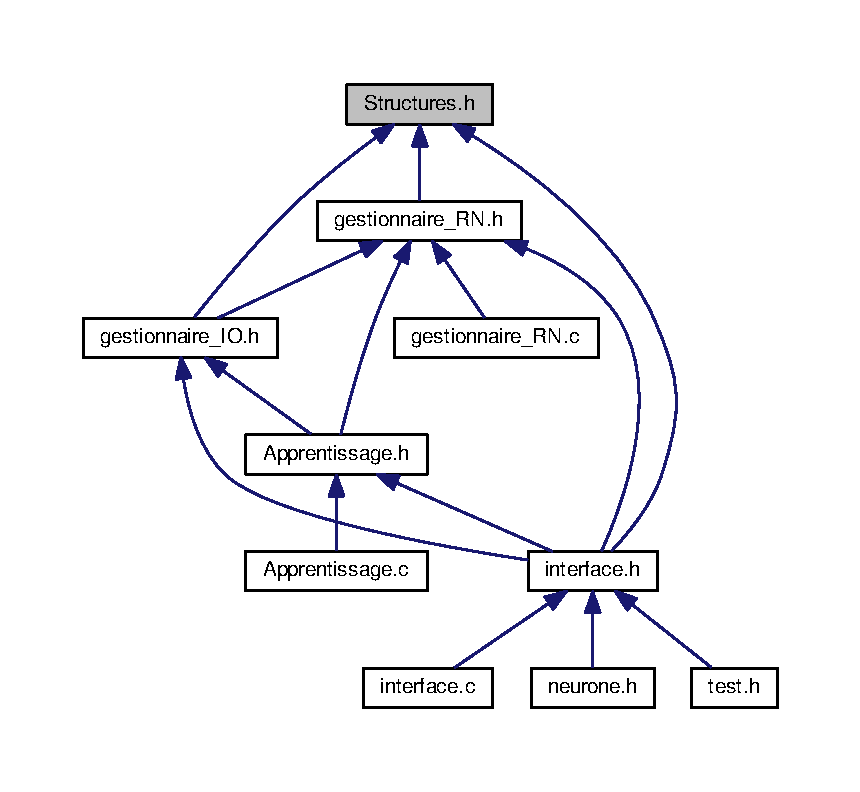
\includegraphics[width=349pt]{Structures_8h__dep__incl}
\end{center}
\end{figure}
\subsection*{Classes}
\begin{DoxyCompactItemize}
\item 
struct \hyperlink{structPixel}{Pixel}
\item 
struct \hyperlink{structImage}{Image}
\item 
struct \hyperlink{structCOUCHE}{C\+O\+U\+C\+HE}
\item 
struct \hyperlink{structINFO__RN}{I\+N\+F\+O\+\_\+\+RN}
\item 
struct \hyperlink{structRN}{RN}
\item 
struct \hyperlink{structApprentissage}{Apprentissage}
\end{DoxyCompactItemize}
\subsection*{Macros}
\begin{DoxyCompactItemize}
\item 
\#define {\bfseries debug}~printf(\char`\"{}line \+: \%d in function \+: \%s in file \%s\textbackslash{}n\char`\"{},\+\_\+\+\_\+\+L\+I\+N\+E\+\_\+\+\_\+,\+\_\+\+\_\+func\+\_\+\+\_\+,\+\_\+\+\_\+\+F\+I\+L\+E\+\_\+\+\_\+);\hypertarget{Structures_8h_a322565ccf348d13e4d3de13af771e5fc}{}\label{Structures_8h_a322565ccf348d13e4d3de13af771e5fc}

\end{DoxyCompactItemize}
\subsection*{Définitions de type}
\begin{DoxyCompactItemize}
\item 
typedef struct \hyperlink{structPixel}{Pixel} {\bfseries Pixel}\hypertarget{Structures_8h_a852667dea7b3568b4439cfa1609f9684}{}\label{Structures_8h_a852667dea7b3568b4439cfa1609f9684}

\item 
typedef struct \hyperlink{structImage}{Image} {\bfseries Image}\hypertarget{Structures_8h_a9082e6aa9fd1705dc218cf44bc5a9d66}{}\label{Structures_8h_a9082e6aa9fd1705dc218cf44bc5a9d66}

\item 
typedef struct \hyperlink{structCOUCHE}{C\+O\+U\+C\+HE} {\bfseries C\+O\+U\+C\+HE}\hypertarget{Structures_8h_a5dc0f579bcb2450225fb26ec264d4964}{}\label{Structures_8h_a5dc0f579bcb2450225fb26ec264d4964}

\item 
typedef \hyperlink{structCOUCHE}{C\+O\+U\+C\+HE} $\ast$ {\bfseries Liste\+\_\+\+Couche}\hypertarget{Structures_8h_a876ff0013427b5aedf2de99fb60d288b}{}\label{Structures_8h_a876ff0013427b5aedf2de99fb60d288b}

\item 
typedef struct \hyperlink{structINFO__RN}{I\+N\+F\+O\+\_\+\+RN} {\bfseries I\+N\+F\+O\+\_\+\+RN}\hypertarget{Structures_8h_a3033b0859de542ddb283e96400adbf30}{}\label{Structures_8h_a3033b0859de542ddb283e96400adbf30}

\item 
typedef struct \hyperlink{structRN}{RN} {\bfseries RN}\hypertarget{Structures_8h_a62a585a5469b8daf8ccdd7a170d17508}{}\label{Structures_8h_a62a585a5469b8daf8ccdd7a170d17508}

\item 
typedef struct \hyperlink{structApprentissage}{Apprentissage} {\bfseries App}\hypertarget{Structures_8h_a3366a0af90a196c6ffb203e17e58cd0e}{}\label{Structures_8h_a3366a0af90a196c6ffb203e17e58cd0e}

\end{DoxyCompactItemize}


\subsection{Description détaillée}
Code contenant les structures utilisées dans le programme. 

\begin{DoxyAuthor}{Auteur}
P\+E\+P\+IN Thibaut 

R\+E\+Z\+G\+UI Soumia 

S\+L\+I\+M\+A\+NI Arezki 

S\+E\+L\+A\+Q\+U\+ET Severine 

S\+Z\+U\+L\+EK Isaac 

M\+O\+N\+T\+I\+G\+N\+ET Anthony 
\end{DoxyAuthor}

%--- End generated contents ---

% Index
\backmatter
\newpage
\phantomsection
\clearemptydoublepage
\addcontentsline{toc}{chapter}{Index}
\printindex

\end{document}
